%Part of/Parte di https://github.com/f-dinucci/appuntiMeccanicaFluidi/
%License/Licenza Creative Commons Attribution-ShareAlike 4.0 International (CC BY-SA 4.0) - attribution/attribuzione Francesco Di Nucci
%See also/Vedere anche https://creativecommons.org/licenses/by-sa/4.0/ and/e https://creativecommons.org/licenses/by-sa/4.0/legalcode
%
\section{Soluzioni esatte equazioni di Navier-Stokes} 
In alcuni casi è possibile trovare delle soluzioni esatte per le equazioni di Navier-Stokes.
Si parte dalle equazioni generali per il caso incomprimibile, la prima semplificazione è di considerare la suddivisione della pressione in ``statica'' e ``dinamica''. 
Questo permette di non tenere  conto della gravità, dato che nelle equazioni rimarrà solamente la pressione dinamica, l'effetto della pressione statica andrà calcolato separatamente:
%
	\begin{equation*}
		\begin{gathered}
			u_x + v_y = 0\\
			u_t + u u_x + v u_y - \frac{1}{\rho} p_x = \nu (u_{xx} + u_{yy}) + \cancel{g_x}\\
			v_t + u v_x + v v_y + \frac{1}{\rho} p_y = \nu (v_{xx} + v_{yy}) + \cancel{g_y}
		\end{gathered}
	\end{equation*}
%

%SUBSECTION
\subsection{Flusso di Pouiseuille piano}
La geometria più semplice possibile è quella con due pareti solide parallele e infinite.
%
	\begin{figure}[ht]
		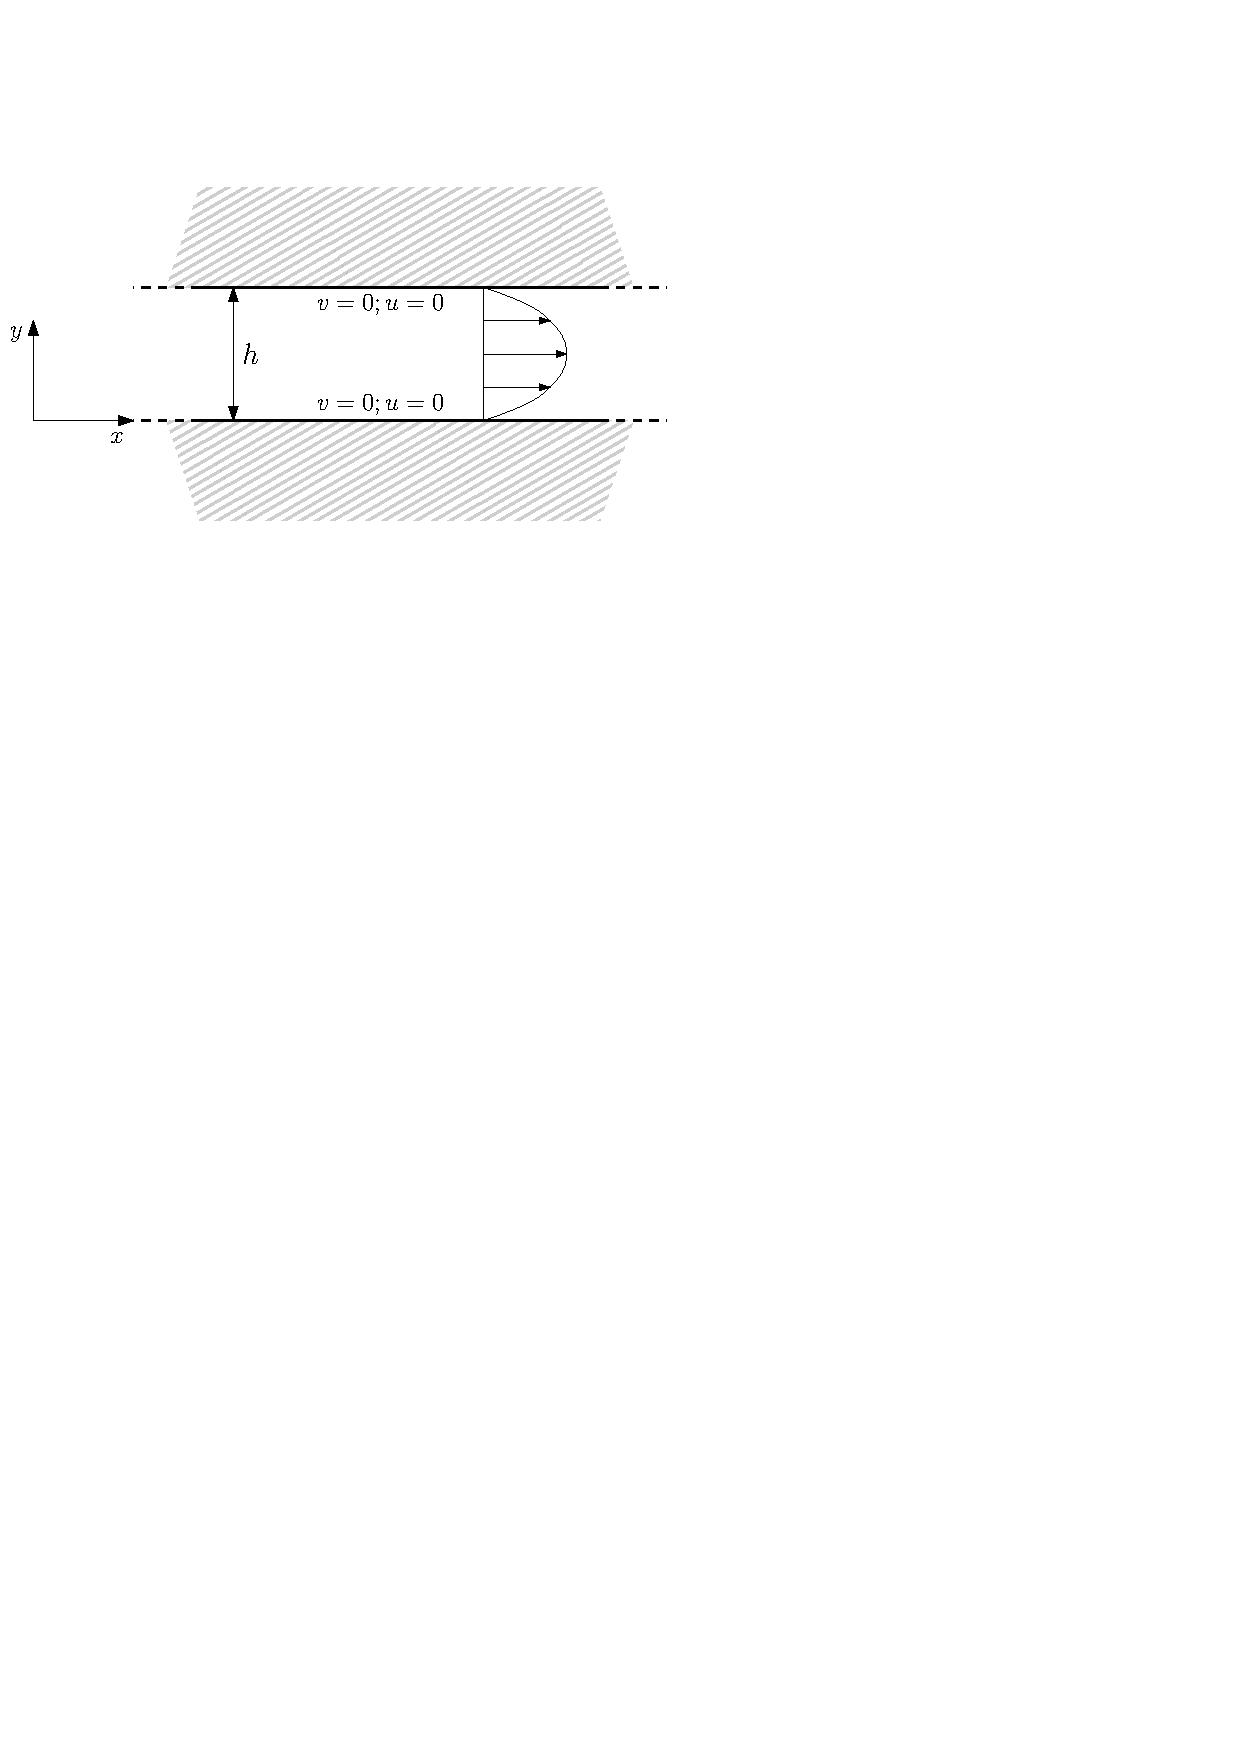
\includegraphics[scale=1.0]{./3.6 Soluzioni esatte equazioni di Navier-Stokes/3.6-1}
		\centering
		\caption{Flusso tra pareti infinite parallele ferme}
	\end{figure}
%
La geometria è indipendente da $x$ e $z$ e si suppone che il sistema sia rimasto a riposo per un periodo sufficientemente lungo per raggiungere la condizione stazionaria, pertanto:
%
	\begin{equation*}
		\pdv{\cdots}{x} = 0 \quad \pdv{\cdots}{t} = 0
	\end{equation*}
%
Dato che la soluzione dipende da una sola variabile è detta ``a moto massimo''.
È invece possibile che ci sia un gradiente di pressione.

Le equazioni di Navier-Stokes quindi diventano:
%
	\begin{equation*}
		\begin{gathered}
			v_y = 0\\
			v u_y + \frac{1}{\rho} p_x = \nu u_{yy}\\
			v v_y + \frac{1}{\rho} p_y = \nu v_{yy}
		\end{gathered}
	\end{equation*}
%
Dalla prima equazione si ricava che la velocità $v$ è costante e dato che alla parete è nulla, è ovunque nulla:
%
	\begin{equation*}
		v_y = 0 \rightarrow v = costante = 0
	\end{equation*}
%
Si arriva quindi a:
%
	\begin{equation*}
		\begin{gathered}
			v_y = 0\\
			\frac{1}{\rho} p_x = \nu u_{yy}\\
			\frac{1}{\rho} p_y = 0
		\end{gathered}
	\end{equation*}
%
Dall'ultima equazione:
%
	\begin{equation*}
		p_y = 0 \rightarrow p_{xy} = 0 \rightarrow p_x = costante
	\end{equation*}
%
Quindi la seconda equazione diventa:
%
	\begin{equation*}
		u_{yy} = \frac{p_x}{\mu}
	\end{equation*}
%
La soluzione è un polinomio di secondo grado:
%
	\begin{equation*}
		u = C_0 + C_1 y + C_2 y^2
	\end{equation*}
%
Calcolando la derivata seconda:
%
	\begin{equation*}
		\begin{gathered}
			\left\{
				\begin{aligned}
					u_{yy} = C_2\\
					u_{yy} = \frac{p_x}{\mu}
				\end{aligned}
			\right.
			\rightarrow C_2 = \frac{p_x}{\mu}
		\end{gathered}
	\end{equation*}
%
Note le condizioni al contorno sulle pareti, si trova il polinomio che le soddisfa (una parabola)\footnote{Questo dimostra che nel calcolo del fattore di correzione ha senso scegliere un profilo parabolico, dato che è soluzione delle equazioni di Navier-Stokes}.
Calcolando poi nuovamente la derivata seconda:
%
	\begin{equation*}
		\begin{gathered}
			u = A y (h - y)\\
			\left\{
				\begin{aligned}
					u_{yy} = -2 A\\
					u_{yy} = \frac{p_x}{\mu}
				\end{aligned}
			\right.
			\rightarrow A = - \frac{p_x}{2 \mu}\\
			\text{quindi}\\
			u = - \frac{p_x}{2 \mu} y (h - y) \quad \textbf{Flusso di Poiseuille}
		\end{gathered}
	\end{equation*}
%
Noto il profilo di velocità è possibile calcolare una serie di grandezze di interesse.

\subsubsection{Velocità massima}
La velocità massima può essere calcolata tramite lo studio della derivata prima oppure si può considerare che dato che il profilo è simmetrico, la velocità massima si troverà al centro, a $y = \frac{h}{2}$:
%
	\begin{equation*}
		u_m = A \frac{h^2}{4} = - \frac{p_x h}{8 \mu}
	\end{equation*}
%
Notare che la pressione diminuisce da sinistra a destra.

\subsubsection{Portata}
La portata può essere calcolata sia in massa che in volume/area, a seconda di se ci sia o meno la densità $\rho$:
%
	\begin{equation*}
		Q = \int_0^h u \dd{y} = A \frac{h^3}{6} = - \frac{p_x h^3}{12 \mu}
	\end{equation*}
%

\subsubsection{Velocità media}
È la velocità che si dovrebbe applicare per avere la stessa portata, è data dal rapporto tra portata e altezza del condotto:
%
	\begin{equation*}
		\bar{u} = \frac{Q}{h} = - \frac{p_x h^2}{12 \mu} = \frac{2}{3} u_m
	\end{equation*}
%

\subsubsection{Sforzo alla parete}
Prendendo a riferimento la parete inferiore, lo sforzo alla parete è dato da:
%
	\begin{equation*}
		\hat{\imath}_x \vdot \uuline{J}_Q \vdot \uline{n} = \hat{\imath}_x \vdot \uuline{J}_Q \vdot (- \hat{\imath}_y) = \tau
	\end{equation*}
%	
Occorre quindi prendere la componente ``fuori diagonale'' del tensore degli sforzi, che viene denominata $\tau$ oppure $\tau_w$\footnote{dato che si trova alla parete, wall}
%
	\begin{equation*}
		\begin{gathered}
			\begin{bmatrix}
				\rho u^2 + p - 2 \mu u_x & \rho u v - \mu (u_y + v_x)\\
				\rho u v - \mu (u_y + v_x) & \rho v^2 + p - 2 \mu v_y\\
			\end{bmatrix}\\
			\text{dato che alla parete la velocità è nulla}\\
			\tau_w = \mu u_y = \mu A h = - h \frac{p_x}{2}
		\end{gathered}
	\end{equation*}
%

%SUBSECTION
\subsection{Flusso di Couette piano}
Si può anche analizzare il caso delle lastre piane parallele nel caso in cui una delle due sia in moto ad una velocità costante $U$, senza un gradiente di pressione.
Notare che normalmente le equazioni di Navier-Stokes sono non lineari, ma avendo in questi casi eliminato i termini non lineari si può applicare il principio di sovrapposizione degli effetti (ad esempio nel caso in cui si abbiano una parete in moto e un gradiente di pressione si possono calcolare separatamente le due soluzioni e sommarne gli effetti).
%
	\begin{figure}[ht]
		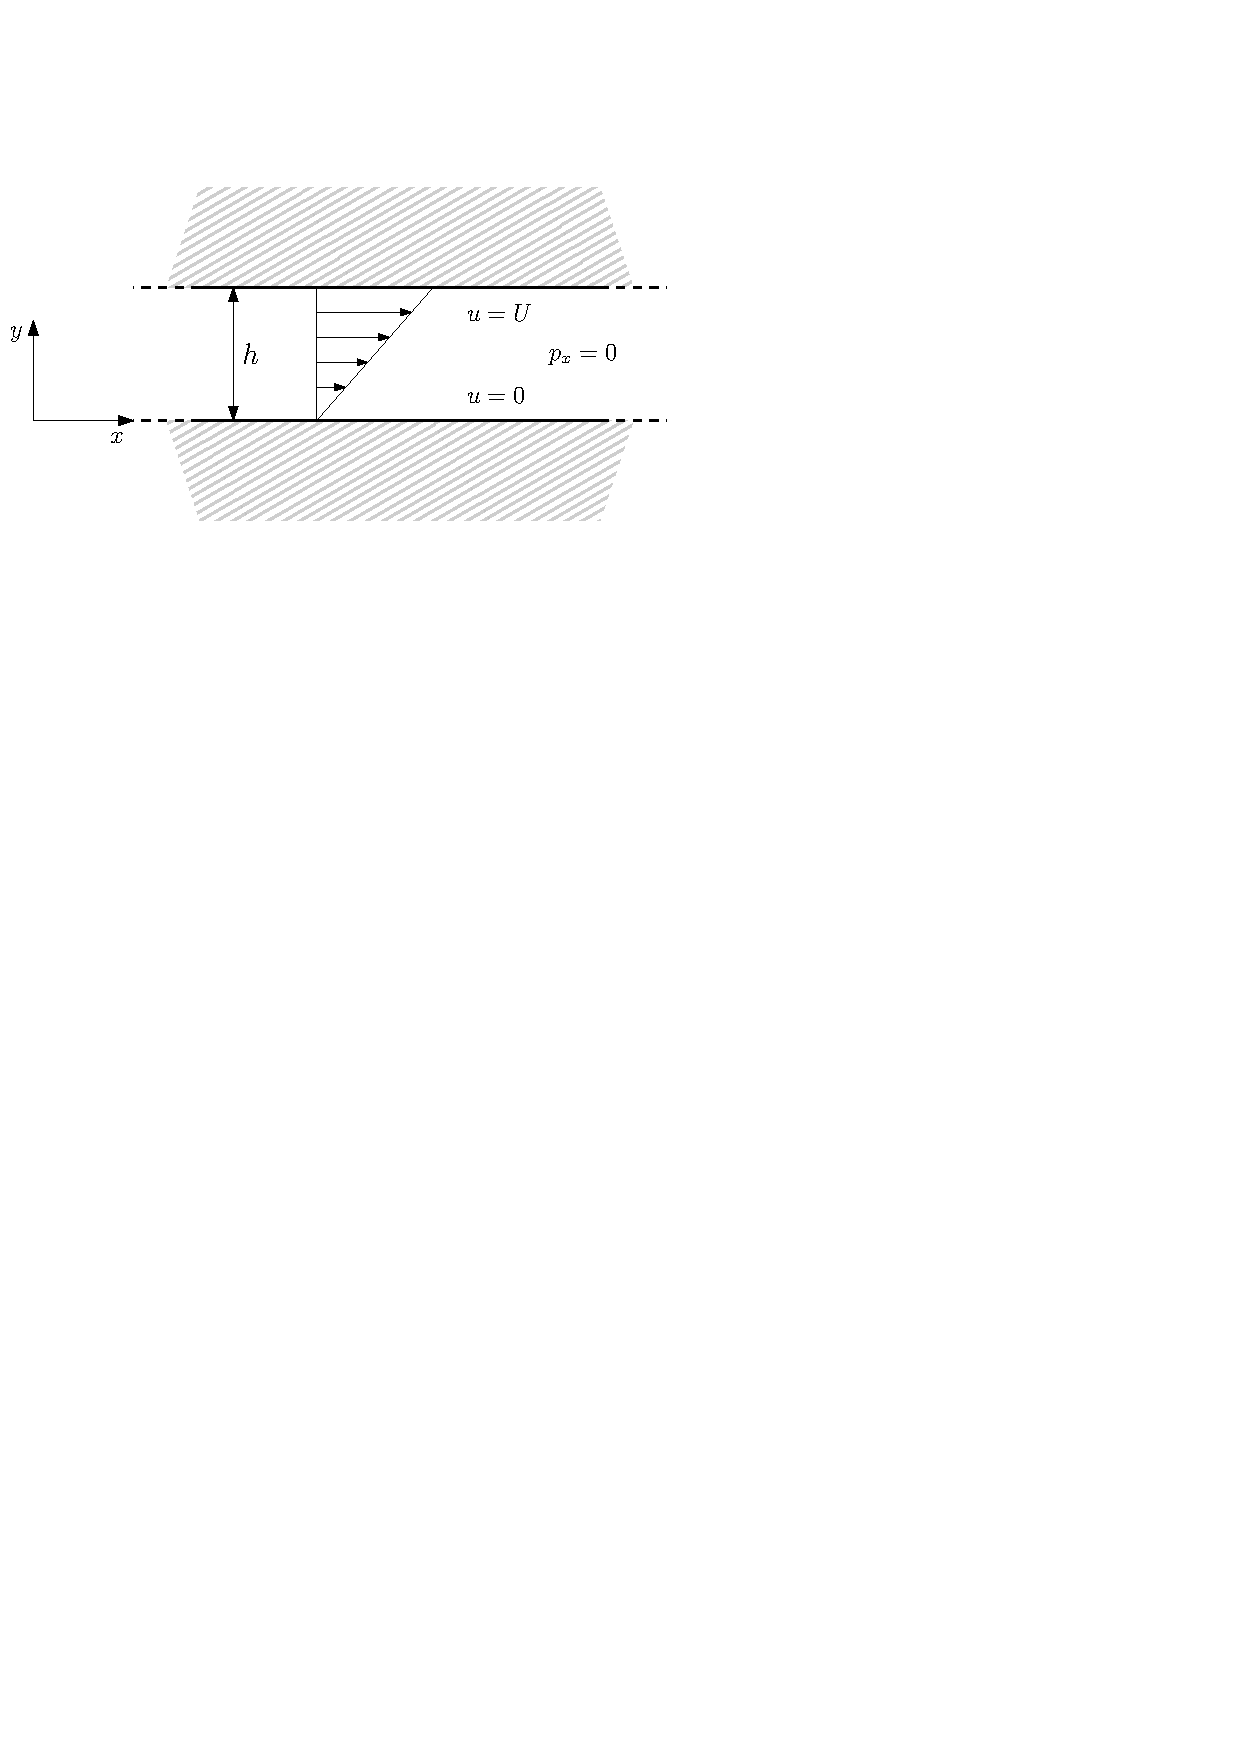
\includegraphics[scale=1.0]{./3.6 Soluzioni esatte equazioni di Navier-Stokes/3.6-2}
		\centering
		\caption{Flusso di Couette piano}
	\end{figure}
%
Poiché si è supposto che non ci sia un gradiente di pressione, $p_x = 0 \rightarrow p_{xy} = 0$, quindi la soluzione è un polinomio di primo grado.
Dalle condizioni al contorno sulle pareti si ricava che:
%
	\begin{equation*}
		u = C_0 + C_1 y = U \frac{y}{h}\\
	\end{equation*}
%

Noto il profilo di velocità è possibile calcolare una serie di grandezze di interesse.

\subsubsection{Velocità massima}
%
	\begin{equation*}
		u_m = U
	\end{equation*}
%

\subsubsection{Velocità media}
%
	\begin{equation*}
		\bar{u} = \frac{U}{2}
	\end{equation*}
%

\subsubsection{Portata}
%
	\begin{equation*}
		Q = h \frac{U}{2}
	\end{equation*}
%

\subsubsection{Sforzo alla parete}
%
	\begin{equation*}
		\tau = \mu u_y = \mu \frac{U}{h}
	\end{equation*}
%

%SUBSECTION
\subsection{Flusso di Pouiseuille cilindrico}
È difficile che si abbia un caso piano, è più frequente che si studi il moto in un condotto.
%
	\begin{figure}[ht]
		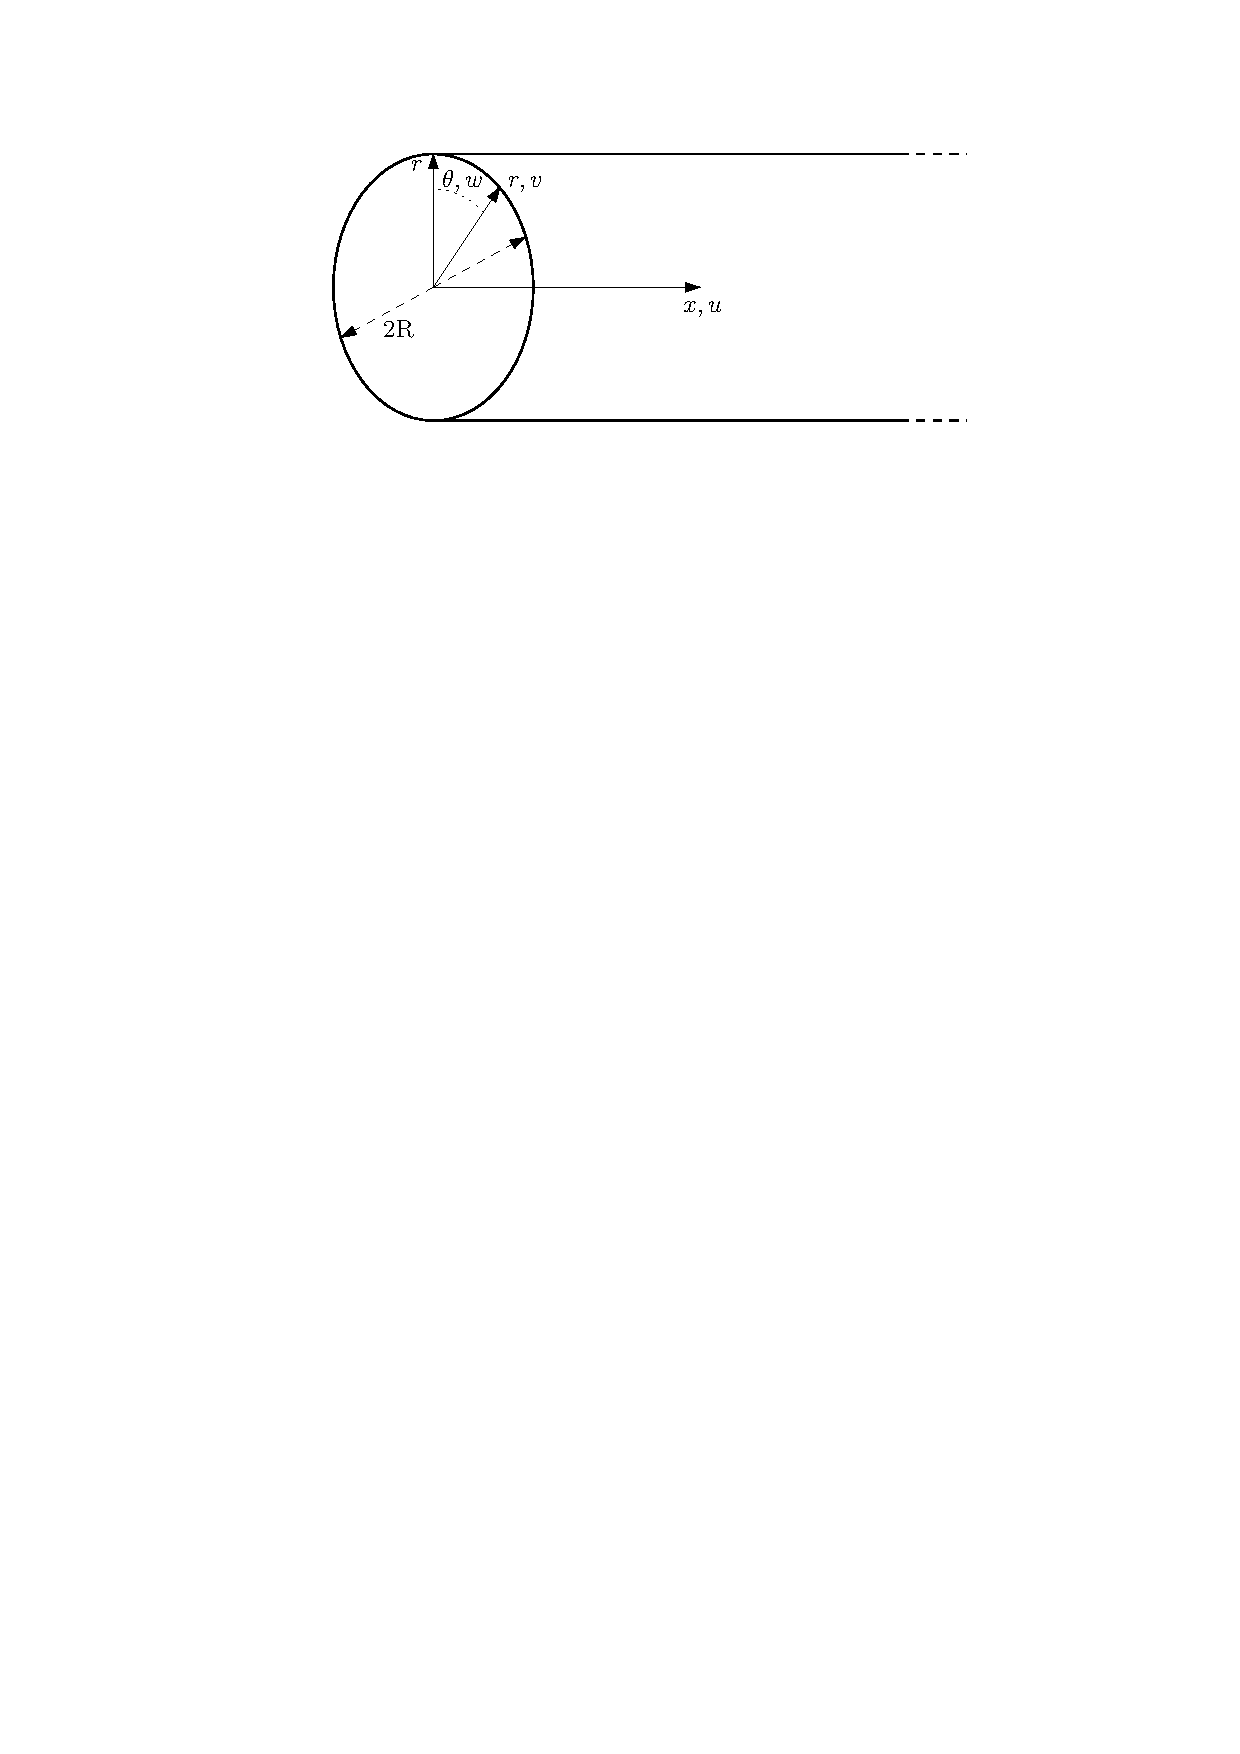
\includegraphics[scale=1.0]{./3.6 Soluzioni esatte equazioni di Navier-Stokes/3.6-3}
		\centering
		\caption{Flusso in condotto}
	\end{figure}
%
Supponendo che ci si trovi a distanza dagli imbocchi la soluzione non dipende da $x$, per simmetria invece non dipende da $\theta$ ed essendo nel caso stazionario non dipende dal tempo:
%
	\begin{equation*}
		\pdv{\cdots}{t} = 0 \quad \pdv{\cdots}{x} = 0 \quad \pdv{\cdots}{\theta} = 0
	\end{equation*}
%

Prese le equazioni in coordinate cilindriche dai testi di riferimento, per l'equazione per la conservazione della massa:
%
	\begin{equation*}
		\begin{gathered}
			\cancel{u_x} + \frac{1}{r} {(rv)}_r + \cancel{\frac{1}{r} w_{\theta}} = 0\\
			\text{poiché la velocità sulla parete è nulla}\\
			rv = costante = 0\\
		\end{gathered}
	\end{equation*}

Le equazioni per la quantità di moto (in coordinate) diventano:
%
	\begin{equation*}
		\begin{gathered}
			\frac{1}{\rho} p_x = \nu \left( \cancel{u_{xx}} + \frac{1}{r} {(r u_r)}_r + \cancel{\frac{1}{r} u_{\theta \theta}} \right)\\
			\frac{1}{\rho} p_{\theta} = 0\\
			- \frac{u^2}{r} + \frac{1}{r} p_r = 0 \rightarrow {\left( - \frac{u^2}{x} \right)}_x + \frac{1}{\rho} p_{rx} = 0 \rightarrow p_x = costante
		\end{gathered}
	\end{equation*}
%
Dalla prima equazione per la quantità di moto si arriva alla soluzione esatta del problema:
%
	\begin{equation*}
		\begin{gathered}
			\frac{1}{r} {(r u_r)}_r = \frac{p_x}{\mu} = costante\\
			{(r u_r)}_r = \frac{p_x}{\mu} r\\
			r u_r = \frac{p_x}{\mu} \frac{r^2}{2} + C_1\\
			u_r = \frac{p_x}{2 \mu} r + \frac{C_1}{r}\\
			u = \frac{p_x}{4 \mu} r^2 + C_1 \log{r}  + C_2
		\end{gathered}
	\end{equation*}
%

Si impongono poi come condizioni al contorno la velocità alla parete ed il fatto che per $r \rightarrow 0$ si ha una ``finta singolarità'', dato che la velocità non può essere infinita:
%
	\begin{equation*}
		\begin{gathered}
			r = R \rightarrow u = 0\\
			r = 0 \quad u \neq \infty \rightarrow C_1 = 0\\
			\text{il polinomio che le rispetta è}\\
			u = A \left( 1 - \frac{r^2}{R^2} \right)\\
		\end{gathered}
	\end{equation*}
Confrontando le due espressioni di $u$:
	\begin{equation*}
		\begin{gathered}
			\left\{
				\begin{aligned}
					u = \frac{p_x}{4 \mu} r^2 + C_1 \log{r}  + C_2\\
					u = A \left( 1 - \frac{r^2}{R^2} \right)
				\end{aligned}
			\right.
			\rightarrow
			A = - \frac{p_x R^2}{4 \mu}\\
			u = - \frac{p_x R^2}{4 \mu} \left( 1 - \frac{r^2}{R^2} \right) \quad \textbf{Flusso di Pouiseuille cilindrico}
		\end{gathered}
	\end{equation*}	
%
Noto il profilo di velocità è possibile calcolare una serie di grandezze di interesse.

\subsubsection{Velocità massima}
%
	\begin{equation*}
		u_m = A
	\end{equation*}
%

\subsubsection{Velocità media}
%
	\begin{equation*}
		\bar{u} = \frac{Q}{\pi R^2} = \frac{A}{2} = - \frac{p_x R^2}{8 \mu}
	\end{equation*}
%

\subsubsection{Portata}
%
	\begin{equation*}
		Q = \int_0^R u 2 \pi r \dd{r} = 2 \pi \int_0^R A \left( 1 - \frac{r^2}{R^2} \right) r \dd{r} = \pi \frac{A R^2}{2}
	\end{equation*}
%

\subsubsection{Sforzo alla parete}
%
	\begin{equation*}
		\tau_{rx} = - \mu u_r = \frac{2 \mu A}{R} = \frac{2 \mu u_m}{R} = \frac{4 \mu \bar{u}}{R} = - \frac{p_x R}{2}
	\end{equation*}
%

%SUBSECTION
\subsection{Flusso di Couette cilindrico}
Si può anche studiare il caso di due cilindrici concentrici, uno dei due in moto longitudinale rispetto all'altro.
%
	\begin{figure}[ht]
		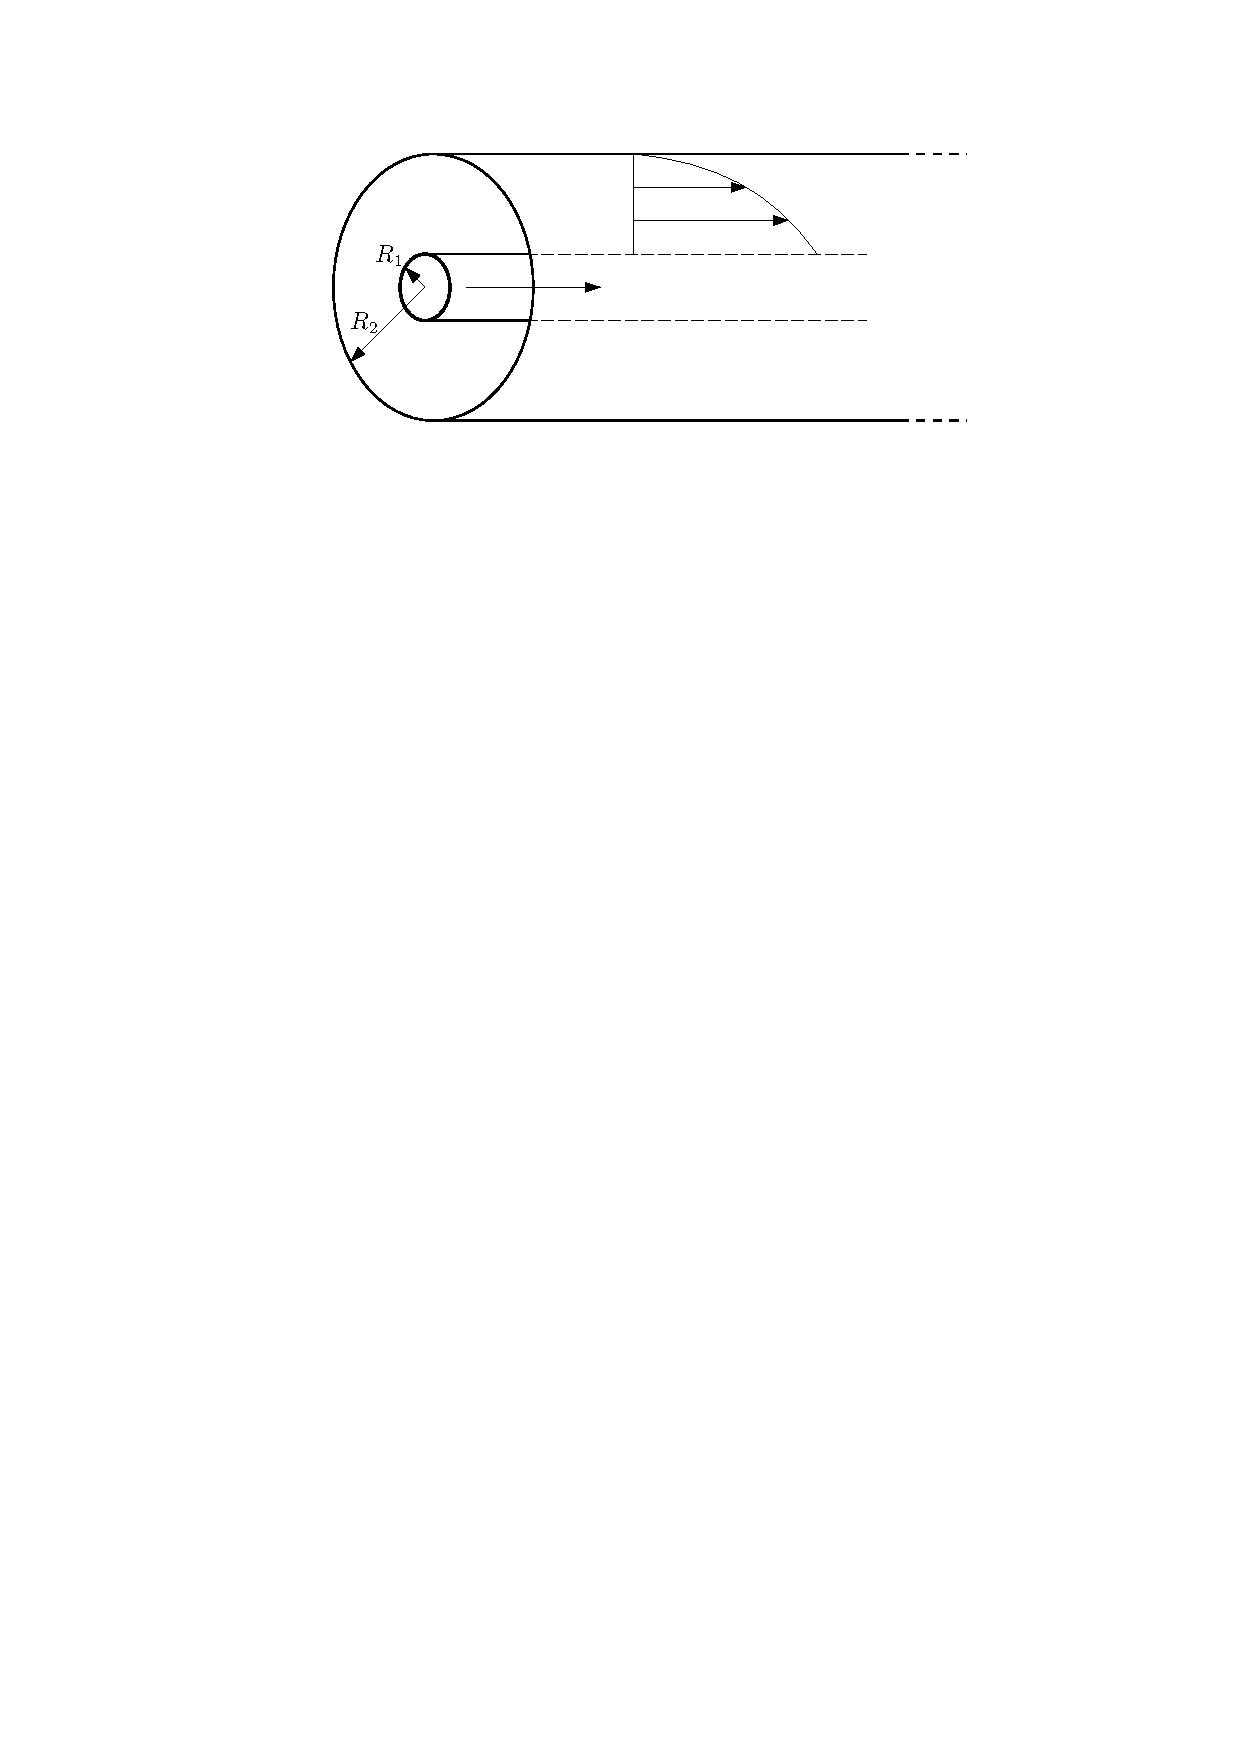
\includegraphics[scale=1.0]{./3.6 Soluzioni esatte equazioni di Navier-Stokes/3.6-4}
		\centering
		\caption{Cilindri concentrici}
	\end{figure}
%
Come soluzione si prende quella del caso precedente:
%
	\begin{equation*}
		u = \frac{p_x}{4 \mu} r^2 + C_1 \log{r} + C_2
	\end{equation*}	
%
In un caso in cui non vi sia un gradiente di pressione, le condizioni al contorno sono invece:
%
	\begin{equation*}
		u(R_1) = U_1 \quad u(R_2) = U_2 \quad p_x = 0
	\end{equation*}	
%
Da queste risultano due equazioni in due incognite:
%
	\begin{equation*}
		\begin{gathered}
			\left\{
				\begin{gathered}
					C_1 \log{R_1} + C_2 = U_1\\
					C_1 \log{R_2} + C_2 = U_2
				\end{gathered}
			\right.
			\rightarrow
			\left\{
				\begin{gathered}
					C_1 = \frac{U_2 - U_1}{\log{R_2} - \log{R_1}}\\
					C_2 = U_1 = \frac{U_2 - U_1}{\log{R_2} - \log{R_1}} \log{R_1}
				\end{gathered}
			\right.
		\end{gathered}
	\end{equation*}
%
Quindi il profilo di velocità può essere scritto come:
%
	\begin{equation*}
		\begin{gathered}
			u = \frac{U_2 - U_1}{\log{\frac{R_2}{R_1}}} \log{r} (\log{r} - \log{R_1}) + U_1\\
			u = \frac{U_2 - U_1}{\log{\frac{R_2}{R_1}}} \log{\frac{r}{R_1}} + U_1 \quad \textbf{Flusso di Couette cilindrico}
		\end{gathered}
	\end{equation*}
%

%SUBSETION 
\subsection{Flusso di Couette azimutale}
 Due cilindri concentrici in rotazione tra loro.
 %
	\begin{figure}[ht]
		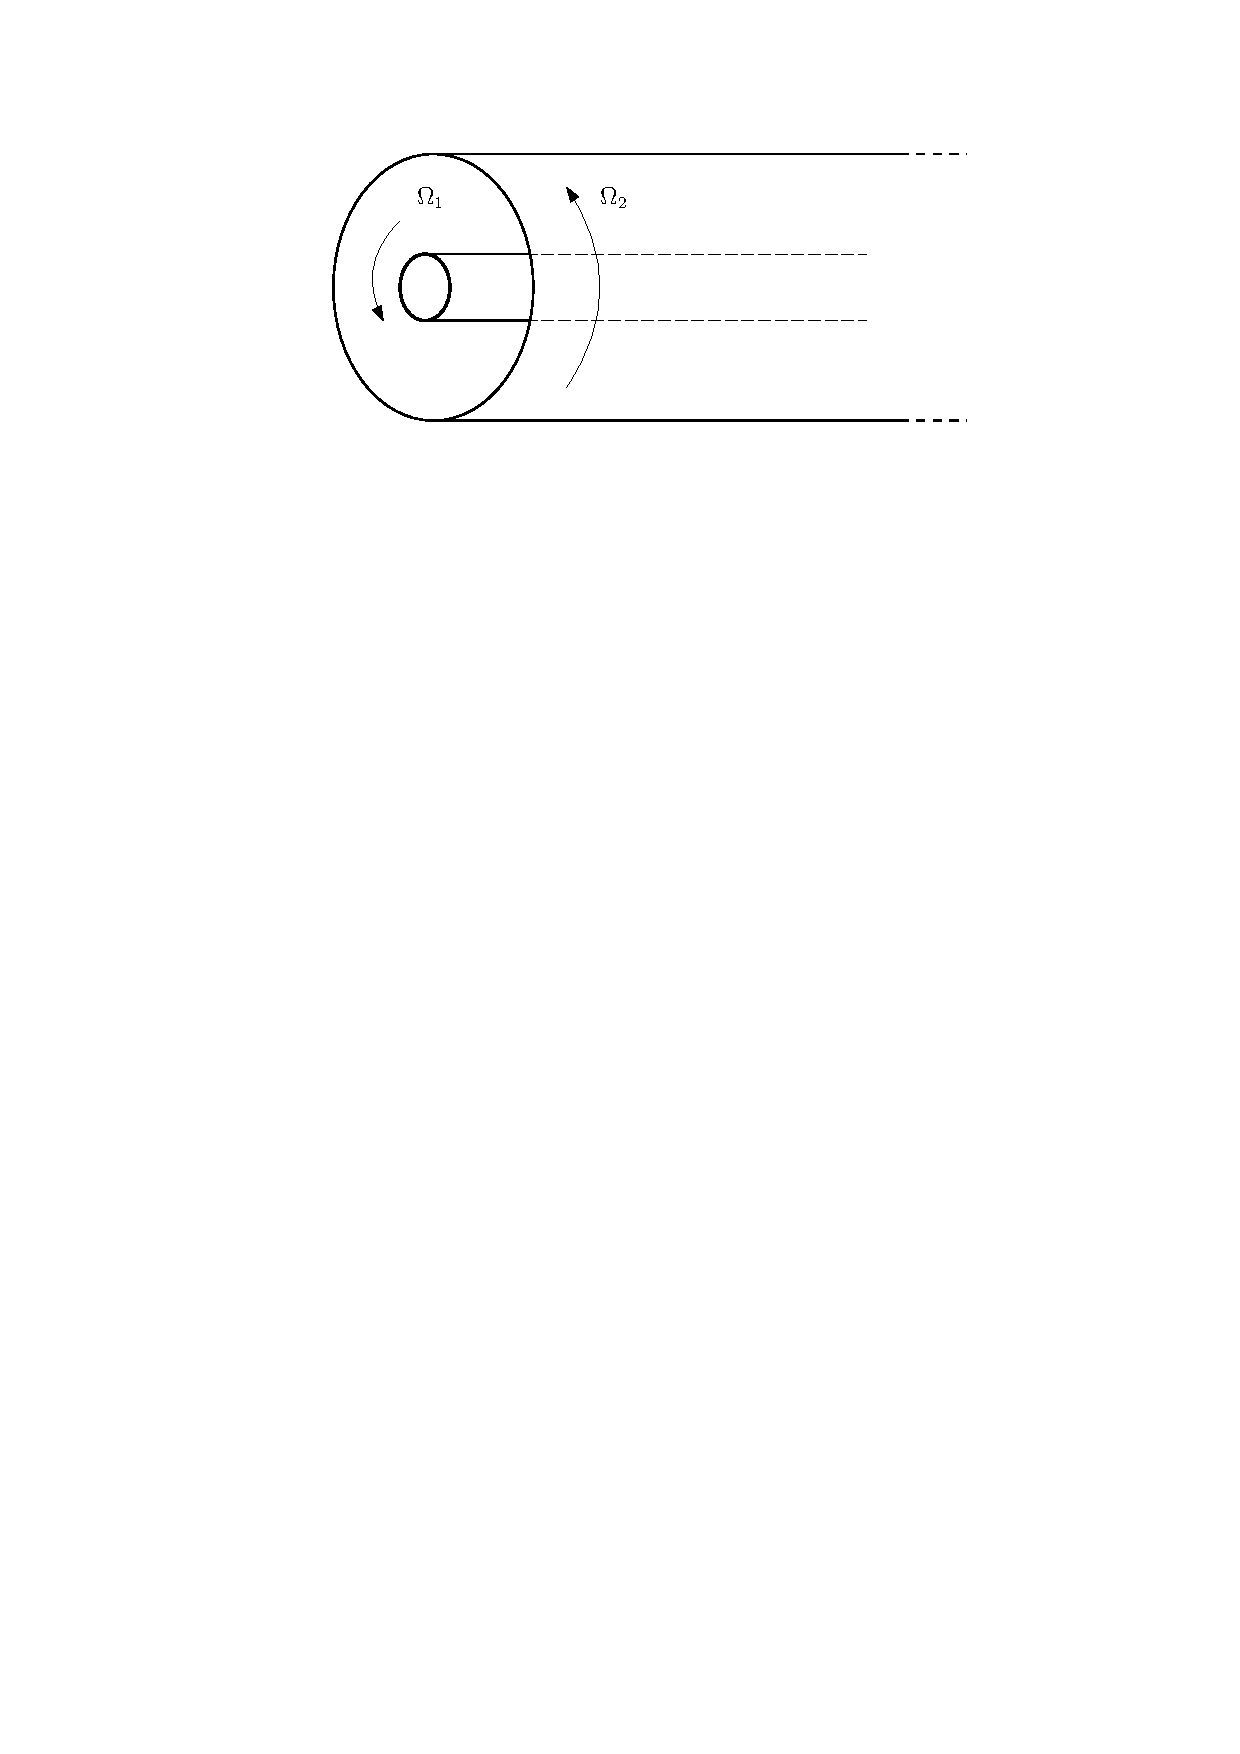
\includegraphics[scale=0.8]{./3.6 Soluzioni esatte equazioni di Navier-Stokes/3.6-5}
		\centering
		\caption{Flusso di Couette azimutale}
	\end{figure}
%
Per simmetria $u = 0$, non c'è differenza tra destra e sinistra del condotto, idem $v = 0$ per l'equazione di continuità.
Si ha quindi che:
	\begin{equation*}
		\begin{gathered}
			\frac{1}{2} {(rv)}_r + \frac{1}{2} w_{\theta} = 0\\
			\text{dove } w = w(r) \rightarrow w_\theta = 0\\
			\frac{1}{2} {(rv)}_r + \cancel{\frac{1}{2} w_{\theta}} = 0\\
			rv = costante\\
			\text{alla parete } v = 0\\
			\text{quindi ovunque}\\
			v = 0
		\end{gathered}
	\end{equation*}

Rimane solamente velocità su w.

I termini che dipendono dal tempo o dalle derivate in $x$ o $\theta$ sono nulli, non c'è la parte convettiva, l'equazione in caso di moto azimutale diventa:
%
	\begin{equation*}
		\frac{1}{2} p_{\theta} = \mu {\left[ \frac{1}{r} {(rw)}_r \right]}_r
	\end{equation*}
%

A confronto nel caso di moto assiale era invece:
%
	\begin{equation*}
		p_x = \mu \frac{1}{r} {(r u_r)}_r
	\end{equation*}
%

Lungo la direzione $\theta$ non può esserci un gradiente di pressione, altrimenti effettuando un giro attorno al cilindro si tornerebbe al punto di partenza, nel quale dovrebbe però esserci una pressione diversa da quella iniziale. 
L'unica soluzione possibile è che non ci sia un gradiente di pressione, in altre parole non esiste un moto di Pouiseuille azimutale.
Quindi:
%
	\begin{equation*}
		\begin{gathered}
			\mu {\left[ \frac{1}{r} {(r w)}_r\right]}_r\\
			\text{integrando}\\
			\frac{1}{r} {(rw)}_r = C_1\\
			{(rw)}_r = C_1 r\\
			rw = C_1 \frac{r^2}{2} + C_2\\
			w = {C'}_1 r + C_2 r^{-1} \quad \text{soluzione del moto}\\
		\end{gathered}
	\end{equation*}
%			
È quindi possibile applicare le condizioni al contorno		
%
	\begin{equation*}
		\begin{gathered}
			\left\{
				\begin{aligned}
					w(R_1) = R_1 {\Omega}_1\\
					w(R_2) = R_2 {\Omega}_2\\
				\end{aligned}
			\right.\\
		\end{gathered}
	\end{equation*}
%
Da queste risulta il sistema:			
%
	\begin{equation*}
		\begin{gathered}			
			\left\{
				\begin{aligned}
					C'_1 R_1 + \frac{C_2}{{R_1}^2} = R_1 {\Omega}_1\\
					C'_1 R_1 + \frac{C_2}{{R_1}^2} = R_2 {\Omega}_2\\
				\end{aligned}
			\right. \\
			\text{le cui soluzioni sono}\\
			{C_1}' = {\Omega}_1 - \frac{{\Omega}_1 - {\Omega}_2}{{R_2}^2 - {R_1}^2}  {R_2}^2\\
			C_2 = \frac{{\Omega}_1 - {\Omega}_2}{{R_2}^2 - {R_1}^2} {R_1}^2 {R_2}^2 \\
		\end{gathered}
	\end{equation*}
%			
Si arriva quindi al \textbf{flusso di Couette azimutale}:
%
	\begin{equation*}	
			w = {C'}_1 r = {\Omega}_1 r - \frac{{\Omega}_1 - {\Omega}_2}{{R_2}^2 - {R_1}^2} {R_2}^2 r + \frac{{\Omega}_1 - {\Omega}_2}{{R_2}^2 - {R_1}^2} {R_1}^2 {R_2}^2 \frac{1}{r}
	\end{equation*}
%

È un profilo che varia in maniera non lineare.
Se i cilindri si muovono alla stessa velocità si torna al caso della rotazione rigida, rimane solamente il termine proporzionale a r.
Se invece il cilindro esterno tende all'infinito (si ha quindi un cilindro in rotazione in fluido illimitato), rimane solamente il termine proporzionale a 1/r.
 %
	\begin{figure}[ht]
		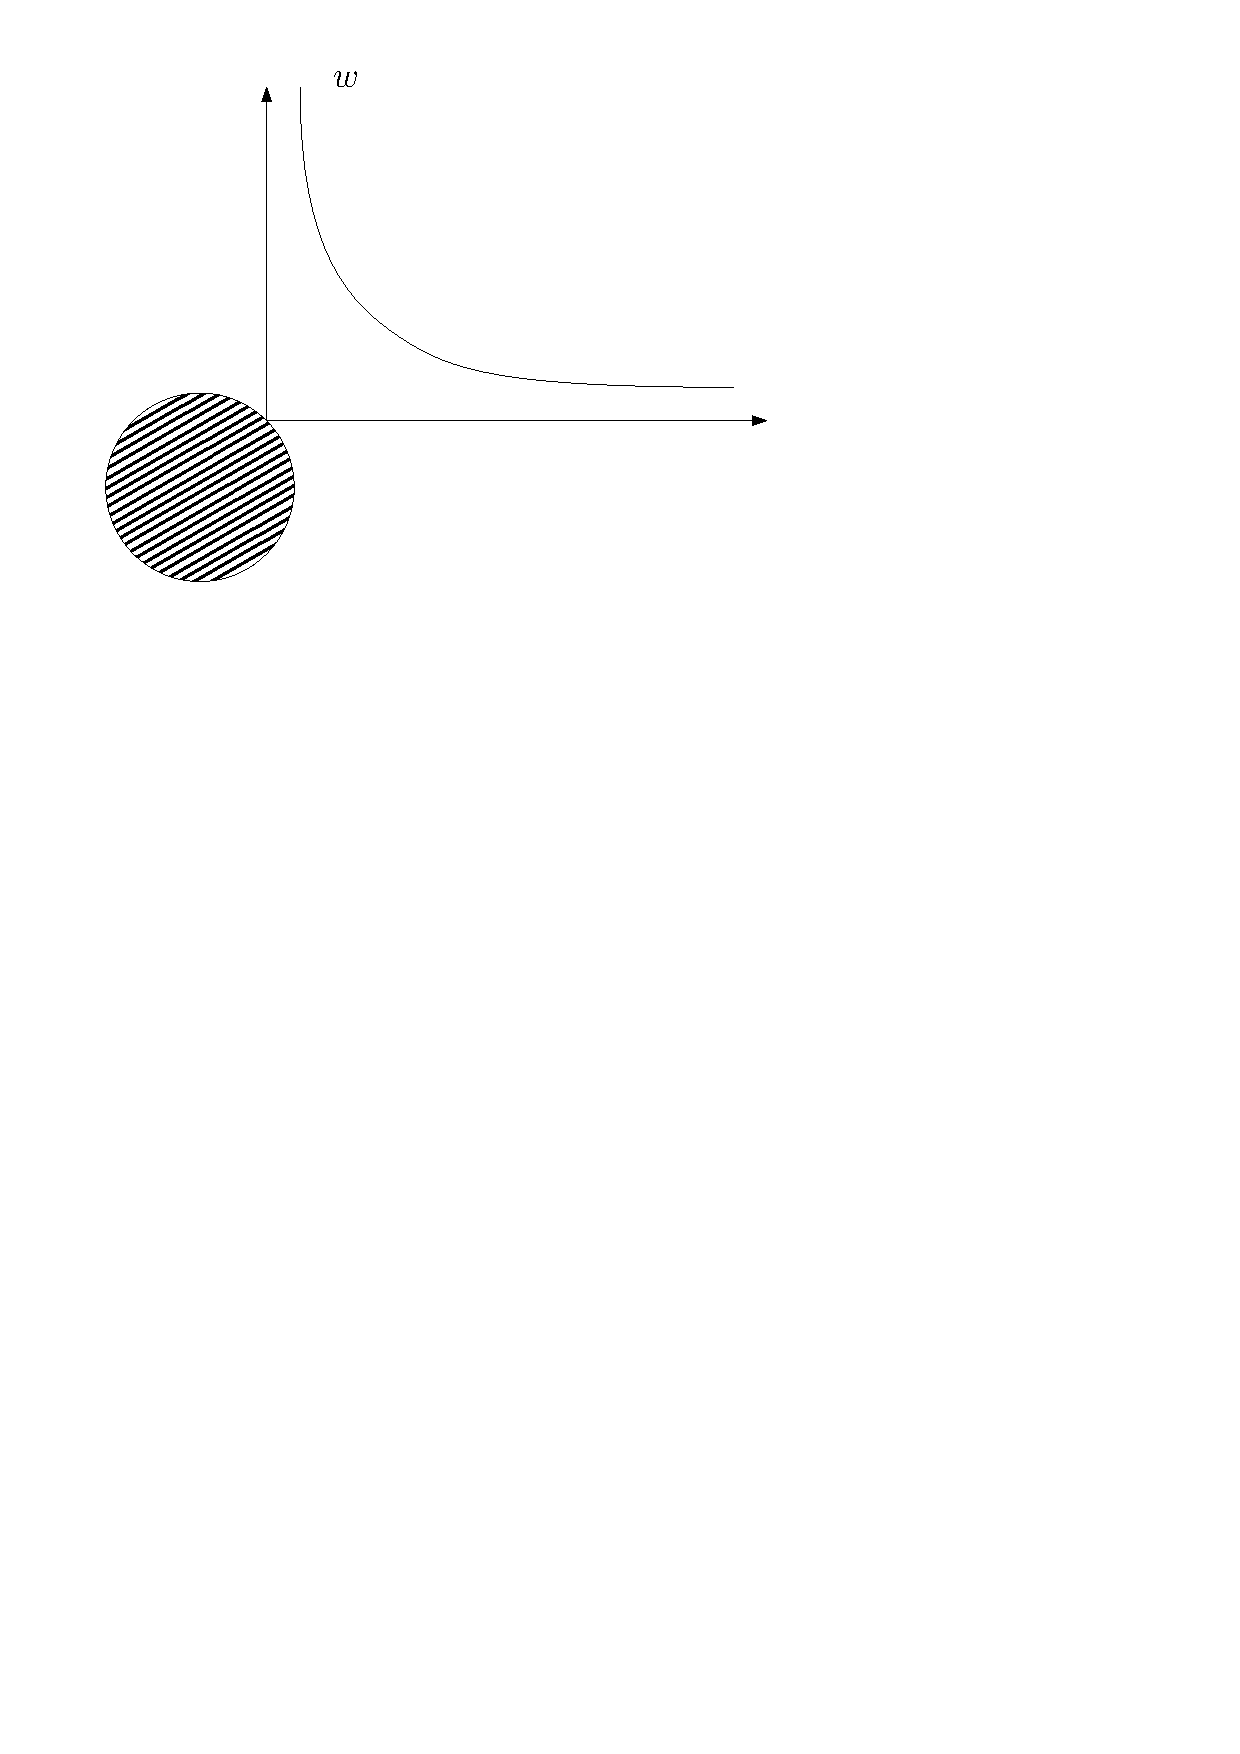
\includegraphics[scale=0.7]{./3.6 Soluzioni esatte equazioni di Navier-Stokes/3.6-6}
		\centering
		\caption{Cilindro in rotazione in fluido illimitato}
	\end{figure}
%

Altro caso che riporta alla rotazione rigida è quello in cui sia presente solamente il cilindro esterno e sia in rotazione, il profilo è lineare in r.
 %
	\begin{figure}[ht]
		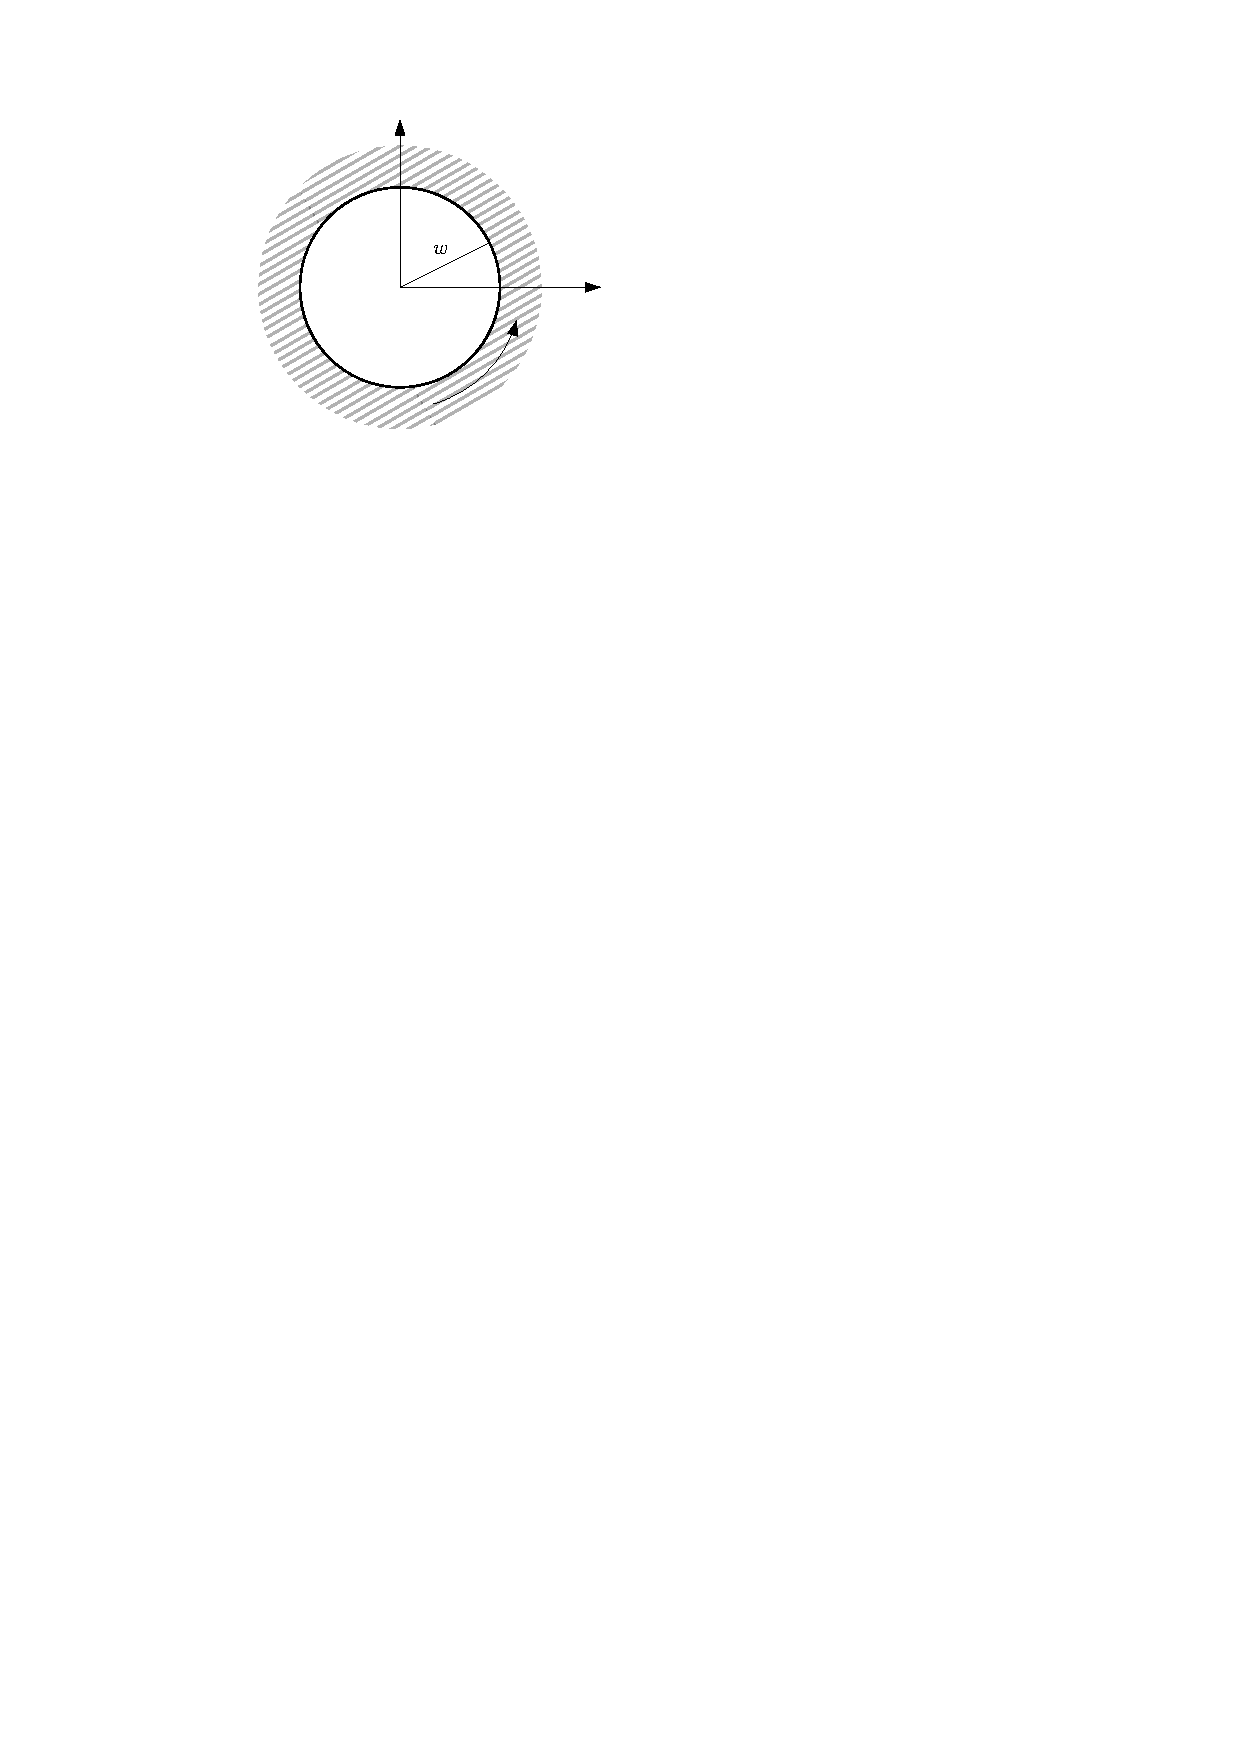
\includegraphics[scale=1.1]{./3.6 Soluzioni esatte equazioni di Navier-Stokes/3.6-7}
		\centering
		\caption{Cilindro pieno di fluido in rotazione}
	\end{figure}
%

È interessante la coppia sulla parete, calcolabile noti lo sforzo di taglio sulla superficie ed il raggio.
Lo sforzo si calcola come:
%
	\begin{equation*}
		\tau = \mu \frac{1}{r} {(rw)}_r
	\end{equation*}
%

 %
	\begin{figure}[ht]
		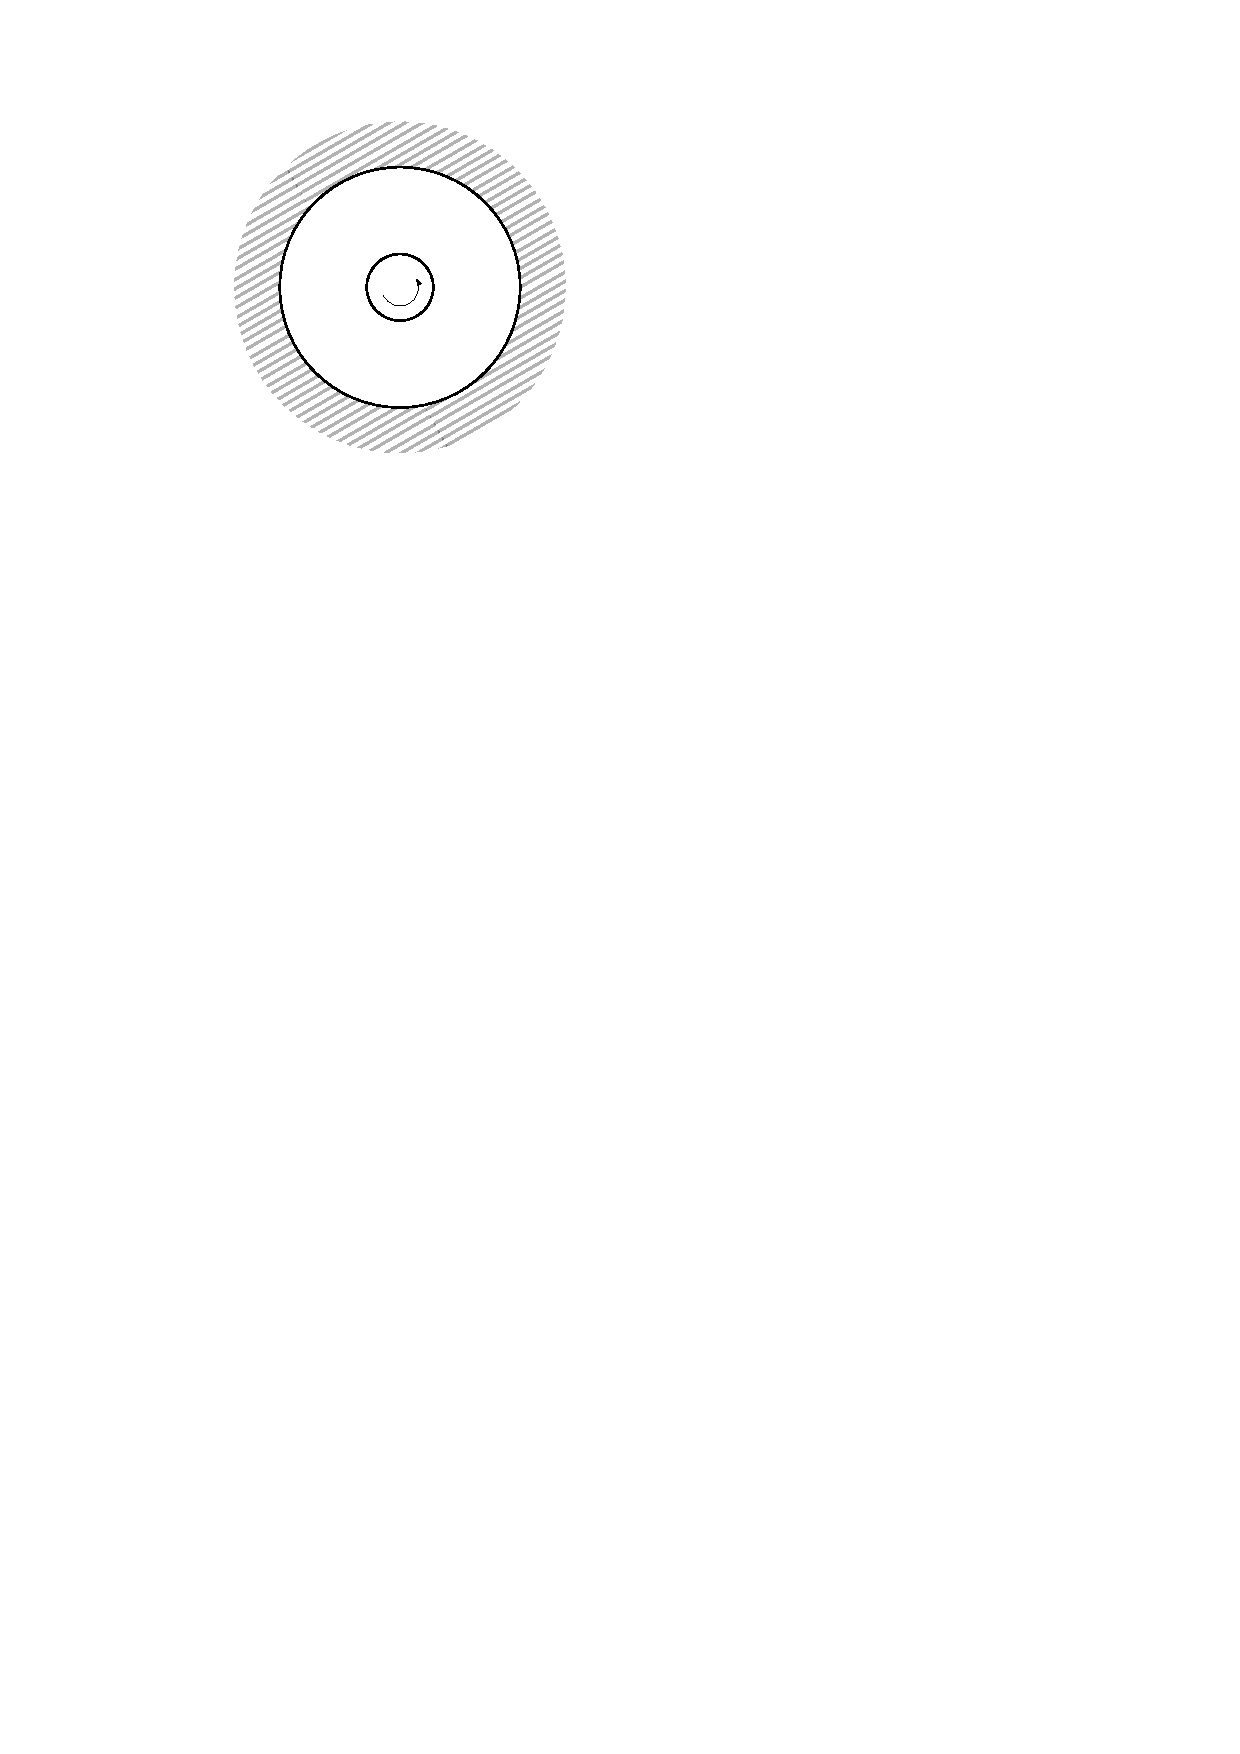
\includegraphics[scale=0.9]{./3.6 Soluzioni esatte equazioni di Navier-Stokes/3.6-8}
		\centering
		\caption{Dinamometro}
	\end{figure}
%
Un esempio di applicazione è il dinamometro, in cui si misura con un dinamometro la coppia necessaria a tenere fermo il cilindro esterno e si ricava il valore della densità.

%SUBSECTION
 \subsection{Problema di Rayleigh}
 Nel problema di Rayleigh si affronta il caso di un moto dipendente anche dal tempo, $u(y,t)$.
In particolare si analizza un caso piano con una sola parete infinita.
Inizialmente la parete è ferma, ad un certo punto inizia a muoversi a velocità costante.


Se la parete fosse in moto stazionario il fluido si muoverebbe con essa e la soluzione sarebbe banale, ma in questo caso si ha che la parete è in moto solamente a partire da un certo istante.
 %
	\begin{figure}[ht]
		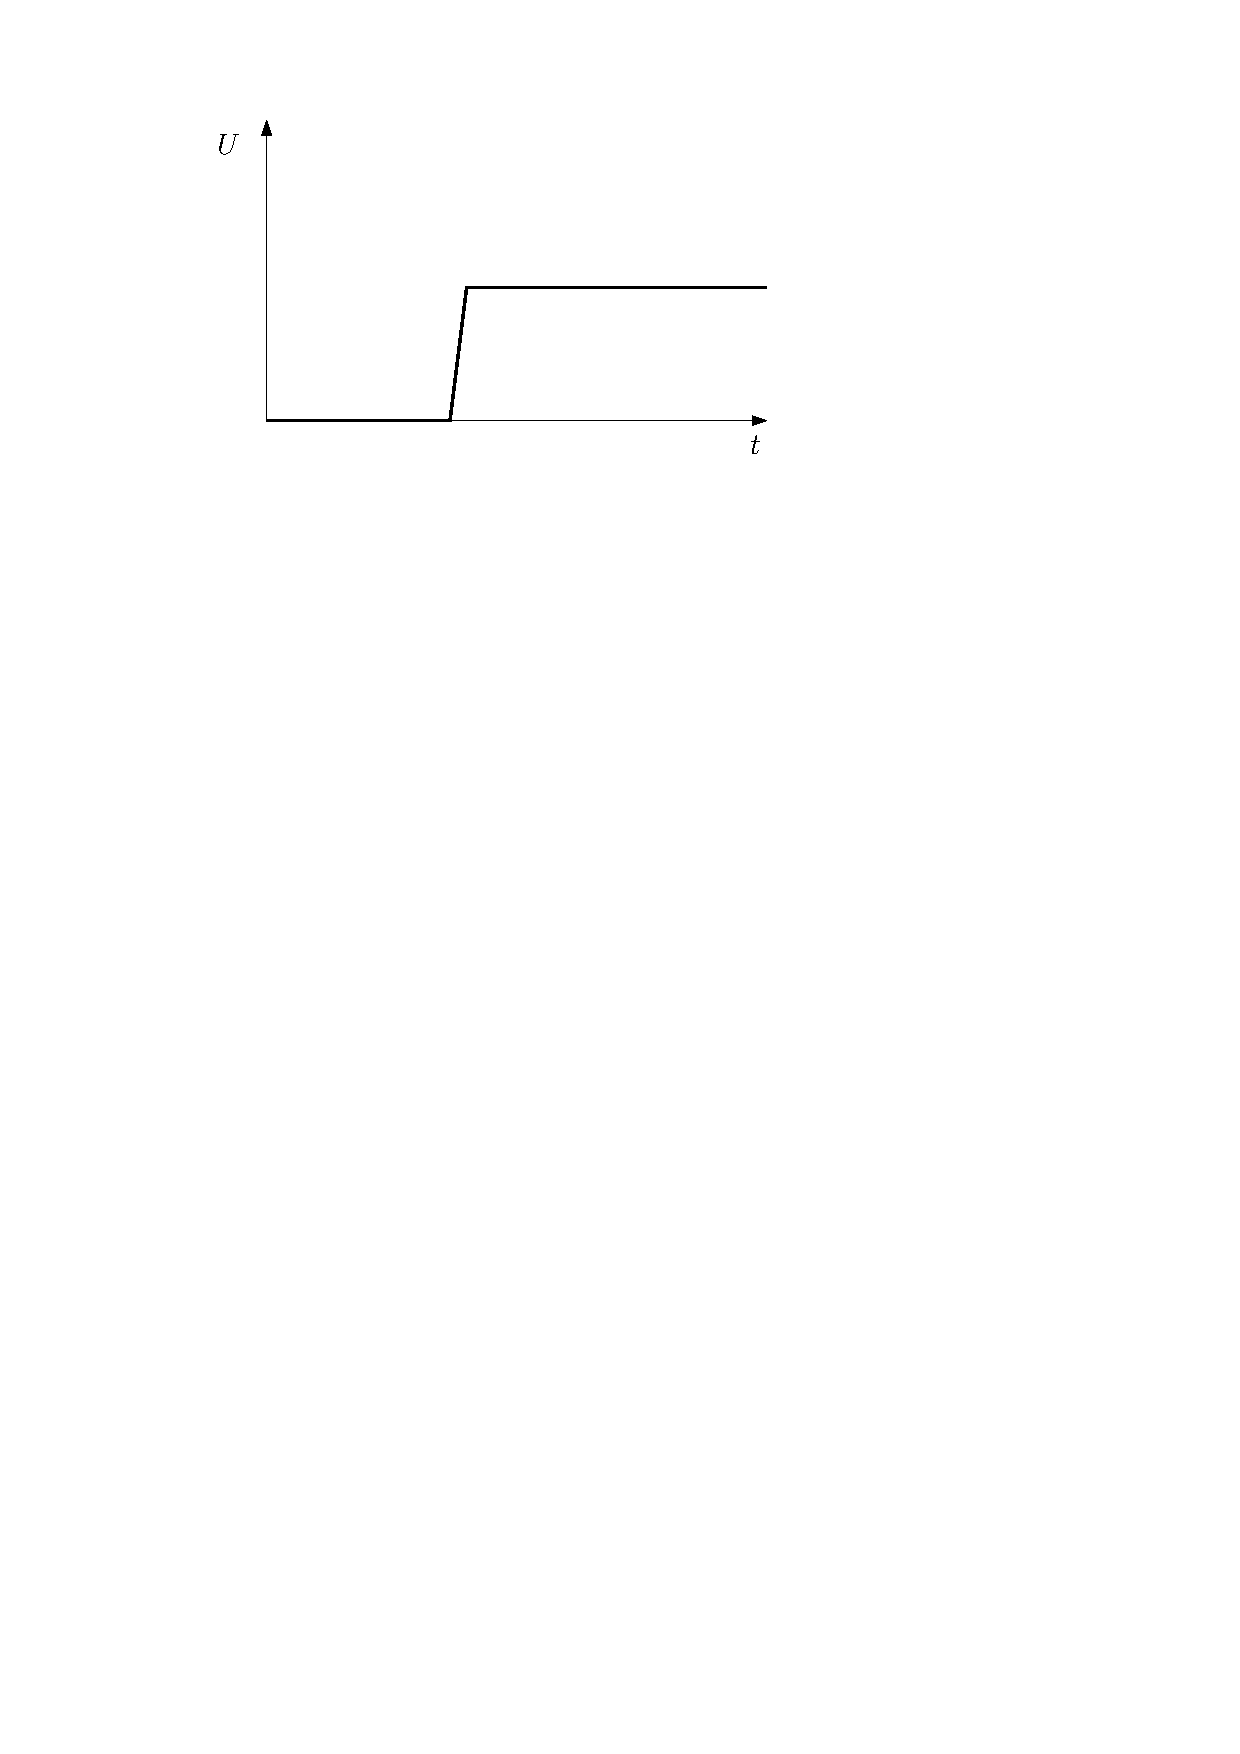
\includegraphics[scale=0.85]{./3.6 Soluzioni esatte equazioni di Navier-Stokes/3.6-9}
		\centering
		\caption{Velocità della parete in funzione del tempo}
	\end{figure}
%

 %
	\begin{figure}[ht]
		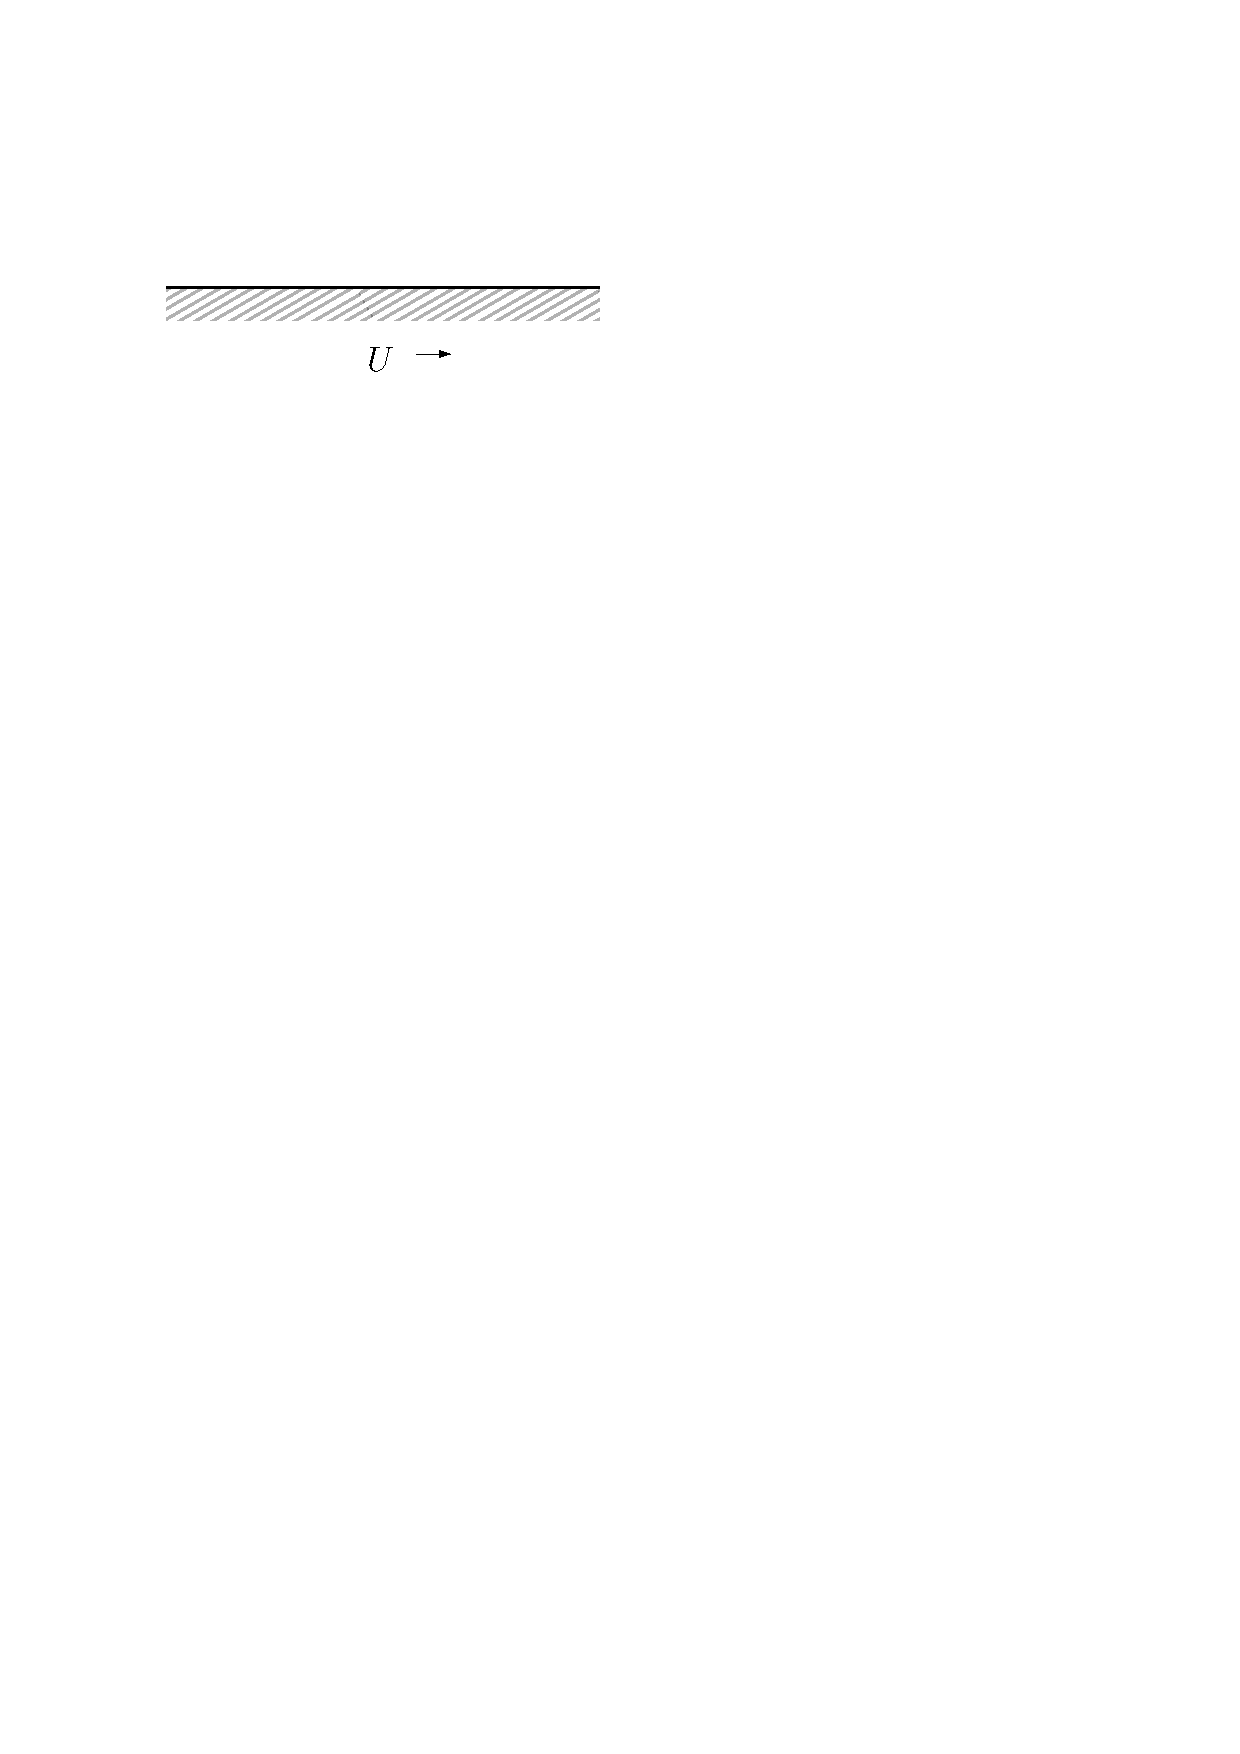
\includegraphics[scale=0.9]{./3.6 Soluzioni esatte equazioni di Navier-Stokes/3.6-10}
		\centering
		\caption{Parete infinita in moto}
	\end{figure}
%

Il ragionamento effettuato nel caso piano sull'equazione di continuità non cambia, $v = 0$.
Nell'equazione per la quantità di moto in questo caso si semplificano nuovamente i termini convettivi, ma non quelli dipendenti dal tempo:
%
	\begin{equation*}
		u_t + \frac{1}{\rho} p_x = \nu u_{yy}
	\end{equation*}
%
Supponendo che non ci sia un gradiente di pressione:
%
	\begin{equation*}
		u_t + \cancel{\frac{1}{\rho} p_x} = \nu u_{yy}
	\end{equation*}
%

Si ottiene un'equazione alle derivate parziali, non ordinaria. 
Non ci sono regole generali di soluzione, solo casi particolari come le ``soluzioni simili/di similitudine'', che permettono di ricondursi ad un'equazione differenziale ordinaria.
In pratica occorre sostituire le derivate fatte con questa ipotesi e vedere se si arriva ad una soluzione.
Si suppone che $u = f \left( \frac{y}{h(t)} \right)$, cioè che sia una funzione di y su scala variabile (il diagramma della y si ``accorcia'' e ``allunga'' di continuo, quindi è `` geometricamente simile'' a se stesso).
Calcolando le derivate:
%
	\begin{equation*}
		\begin{gathered}
			u_y = f' \frac{1}{h}\\
			u_{yy} = \frac{1}{h^2} f''\\
			u_t = f' \left( - \frac{y h'}{h^2} \right)
		\end{gathered}
	\end{equation*}
%	
Sostituendo le derivate:
%
	\begin{equation*}
		\begin{gathered}
			u_t  = \nu u_{yy}\\
			\text{diventa}\\
			- \frac{y h'}{h^2} f' = \nu \frac{1}{h^2} f''\\
		\end{gathered}
	\end{equation*}
%			
In cui:			
%
	\begin{equation*}
		\begin{gathered}
			\left\{
				\begin{aligned}
					h = h(t)\\
					f = f(z)\\
					z = \frac{y}{h} \rightarrow y = zh\\
				\end{aligned}
			\right.\\
			\text{quindi}\\
			-h h' z f' = \nu f''
		\end{gathered}
	\end{equation*}
%
Questa è sia funzione sia del tempo che di $z$, non si può trovare una soluzione.
Si ipotizza allora che la $h$ sia costante e non $h(t)$, che è come un'equazione differenziale a parte:
%
	\begin{equation*}
		\begin{gathered}
			h h' = C\\
			\frac{h^2}{2} = C t + D\\
		\end{gathered}
	\end{equation*}
%
Basta risolvere in un caso, si prendono quindi $D = 0$ e $C = \frac{\nu}{2}$, da cui $h = \nu t^{1/2}$.
Supposto $h h'$ costante si ha solo una funzione di z, una sola variabile.
Quindi sostituendo si ottiene:
	\begin{equation*}
		\begin{gathered}
			- \frac{1}{2} z f' = f''\\
			\text{incognita ausiliaria}\\
			g = f'\\
			- \frac{1}{2} z g = g' = \frac{\dd{g}}{\dd{z}}\\
			- \frac{1}{2} z \dd{z} = \frac{\dd{g}}{g}\\
			\text{Integrando}\\
			- \frac{z^2}{4} = \log{g} + A\\
			\text{da cui}\\
			g = A' e^{- \frac{z^2}{4}}\\
			\text{Integrando per tornare a f}\\
			f = A' \int_0^z e^{- \frac{z^2}{4}} + B
		\end{gathered}
	\end{equation*}
%

Questo integrale non ha una soluzione analitica, è una funzione gaussiana, che si può ricondurre alla funzione degli errori\footnote{alias error function} $\erf{(x)}$.
Questa è definita come:
%
	\begin{equation*}
		\erf{(x)} = \frac{1}{\sqrt{\pi}} \int_0^x e^{-x^2} \dd{x}
	\end{equation*}
%
Si ha che $\erf{(0)} = 0$ e $\erf{(\infty)} = 1$.

Quella trovata prima non è esattamente la funzione degli errori, si definisce quindi $x = \frac{z}{2}$, per potercisi ricondurre, risulta un'altra costante arbitraria A:
	\begin{equation*}
		\begin{gathered}
			u = A \erf{\frac{z}{2}} + B\\
			\text{dove}\\
			z = \frac{y}{\sqrt{\nu t}}
		\end{gathered}
	\end{equation*}
Questa è la soluzione esatta del problema, cui si applicano le condizioni al contorno: a grande distanza il fluido è fermo, all'inizio il fluido è fermo e la lastra si muove a velocità $U$:
%
	\begin{equation*}
		\begin{gathered}
			\left\{
				\begin{aligned}
					u(\infty,t) = 0\\
					u(y, 0) = 0\\
					u(0, t) = U\\
				\end{aligned}
			\right.\\
			u = U \left[ 1 - \erf{\left( \frac{z}{2} \right)} \right] = U \textrm{erfc}\left( \frac{z}{2} \right)
		\end{gathered}
	\end{equation*}
%
Dove erfc è la funzione complementare degli errori, (1 - erf).
 %
	\begin{figure}[ht]
		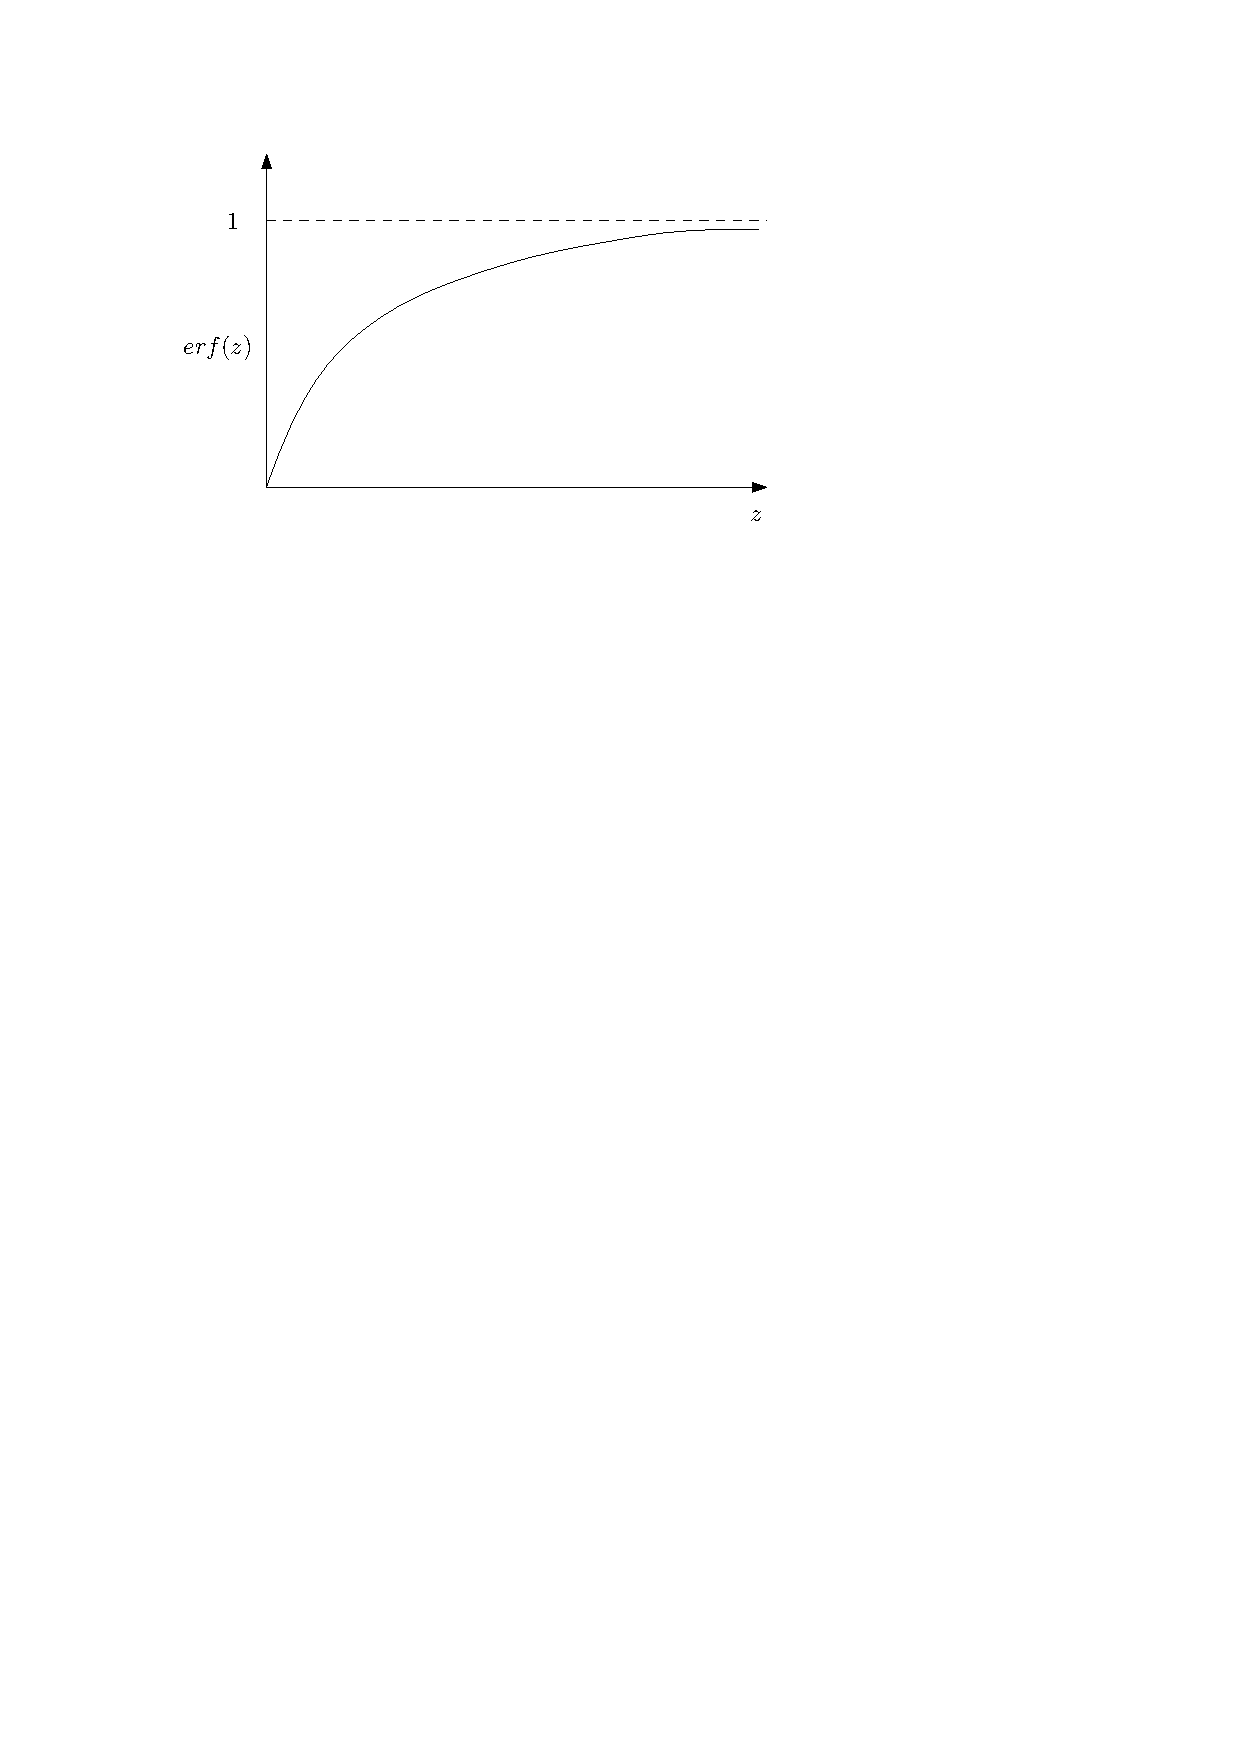
\includegraphics[scale=0.9]{./3.6 Soluzioni esatte equazioni di Navier-Stokes/3.6-11}
		\centering
		\caption{Funzione degli errori}
	\end{figure}
%
La velocità nel tempo va con la funzione complementare degli errori, il cui grafico è circa speculare quello della funzione degli errori.
 %
	\begin{figure}[ht]
		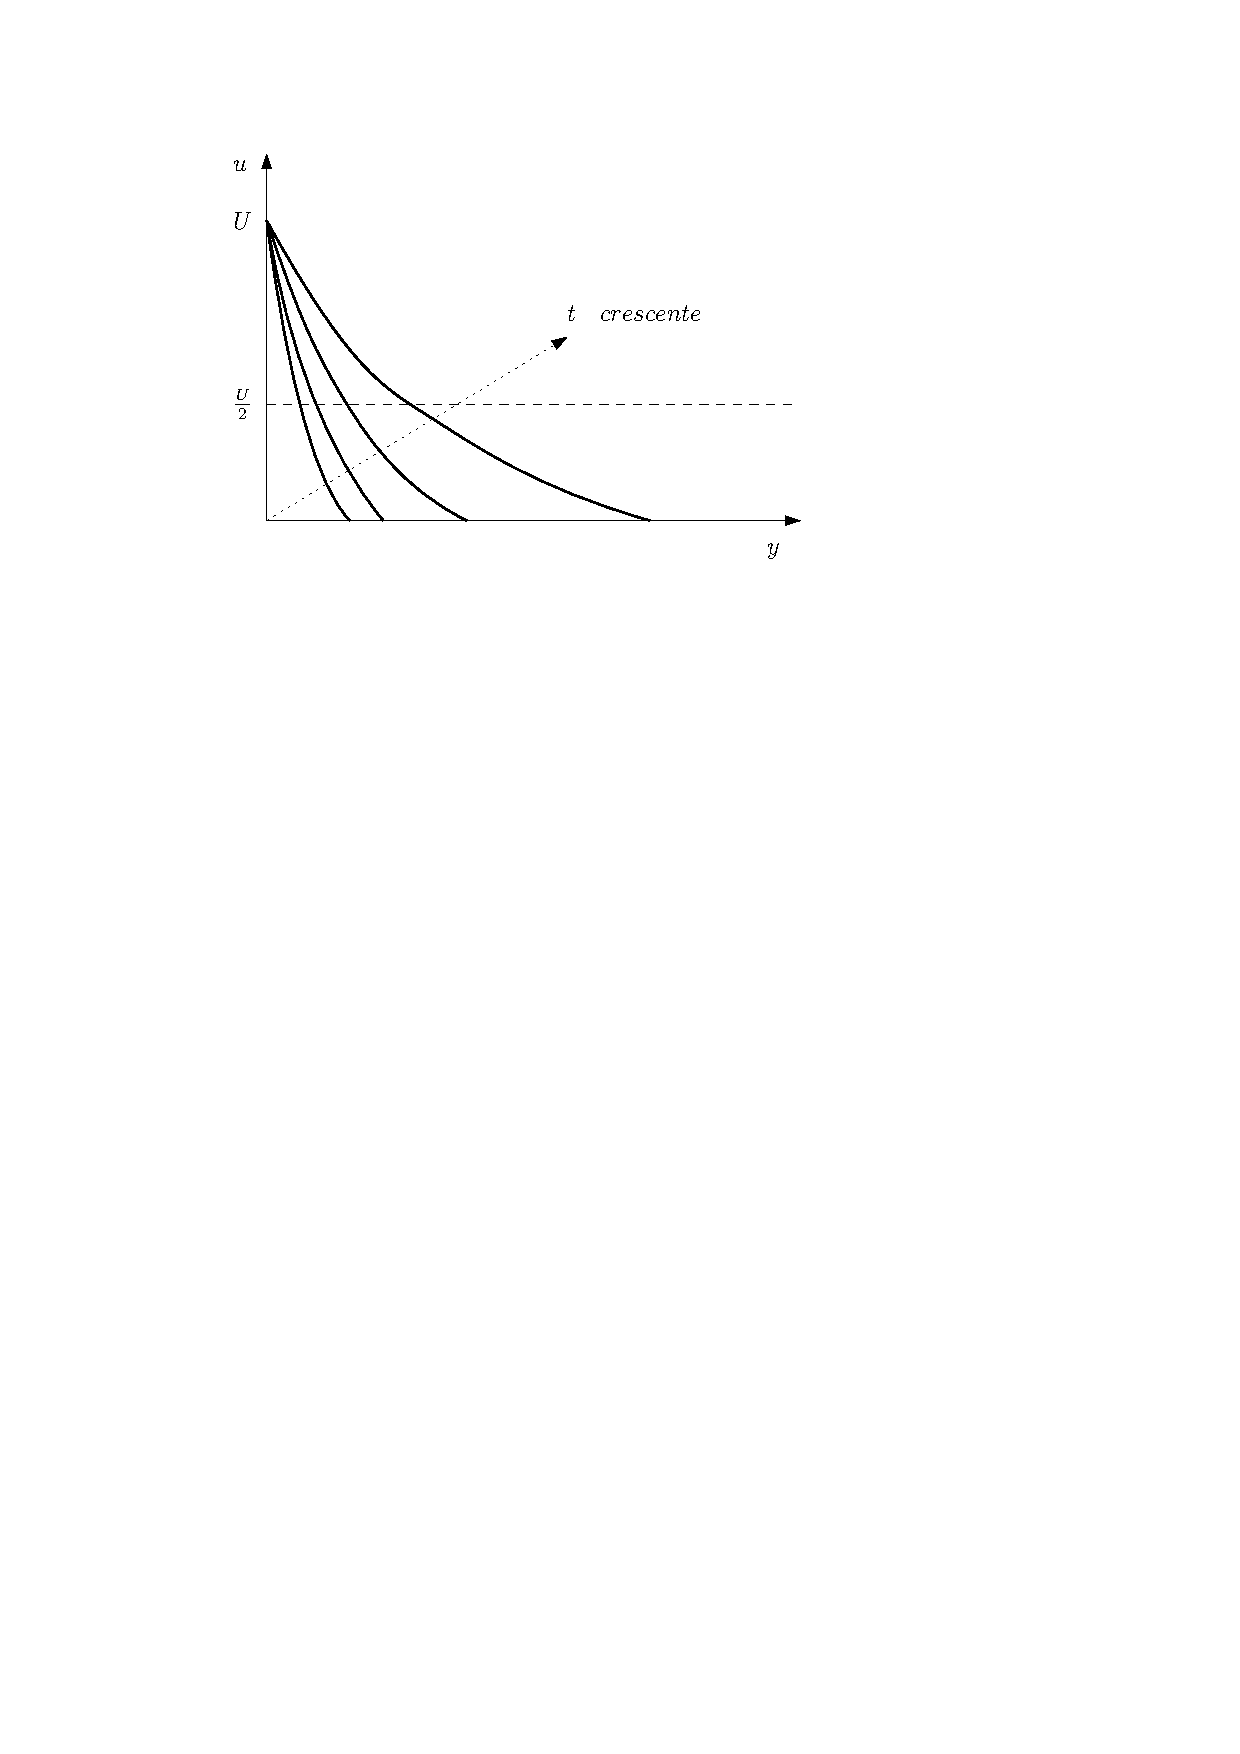
\includegraphics[scale=0.9]{./3.6 Soluzioni esatte equazioni di Navier-Stokes/3.6-12}
		\centering
		\caption{Velocità del fluido nel tempo.}
	\end{figure}
%
Come si può vedere dal grafico, all'inizio il fluido è fermo, poi nel tempo si mette in moto una zona di fluido via via più spessa.
Questa è quantificabile tramite lo spessore, ad esempio si può calcolare la posizione $z_{1/2}$ dove il fluido va alla metà della velocità della parete, $U/2$:
%
	\begin{equation*}
		\erf(z_{1/2}) = \frac{1}{2}
	\end{equation*}
%
Cioè
%
	\begin{equation*}
		y_{1/2} = \sqrt{\nu t} z_{1/2}
	\end{equation*}
%
Sono numeri proporzionali a $\sqrt{\nu t}$, si può ad esempio scegliere $y_{90\%} = \sqrt{\nu t} z_{90 \%}$
Analizzando l'andamento di $y_{1/2}$ in funzione del tempo si vede che lo spessore della zona in moto cresce nel tempo e che il grafico è una parabola rovesciata:
 %
	\begin{figure}[ht]
		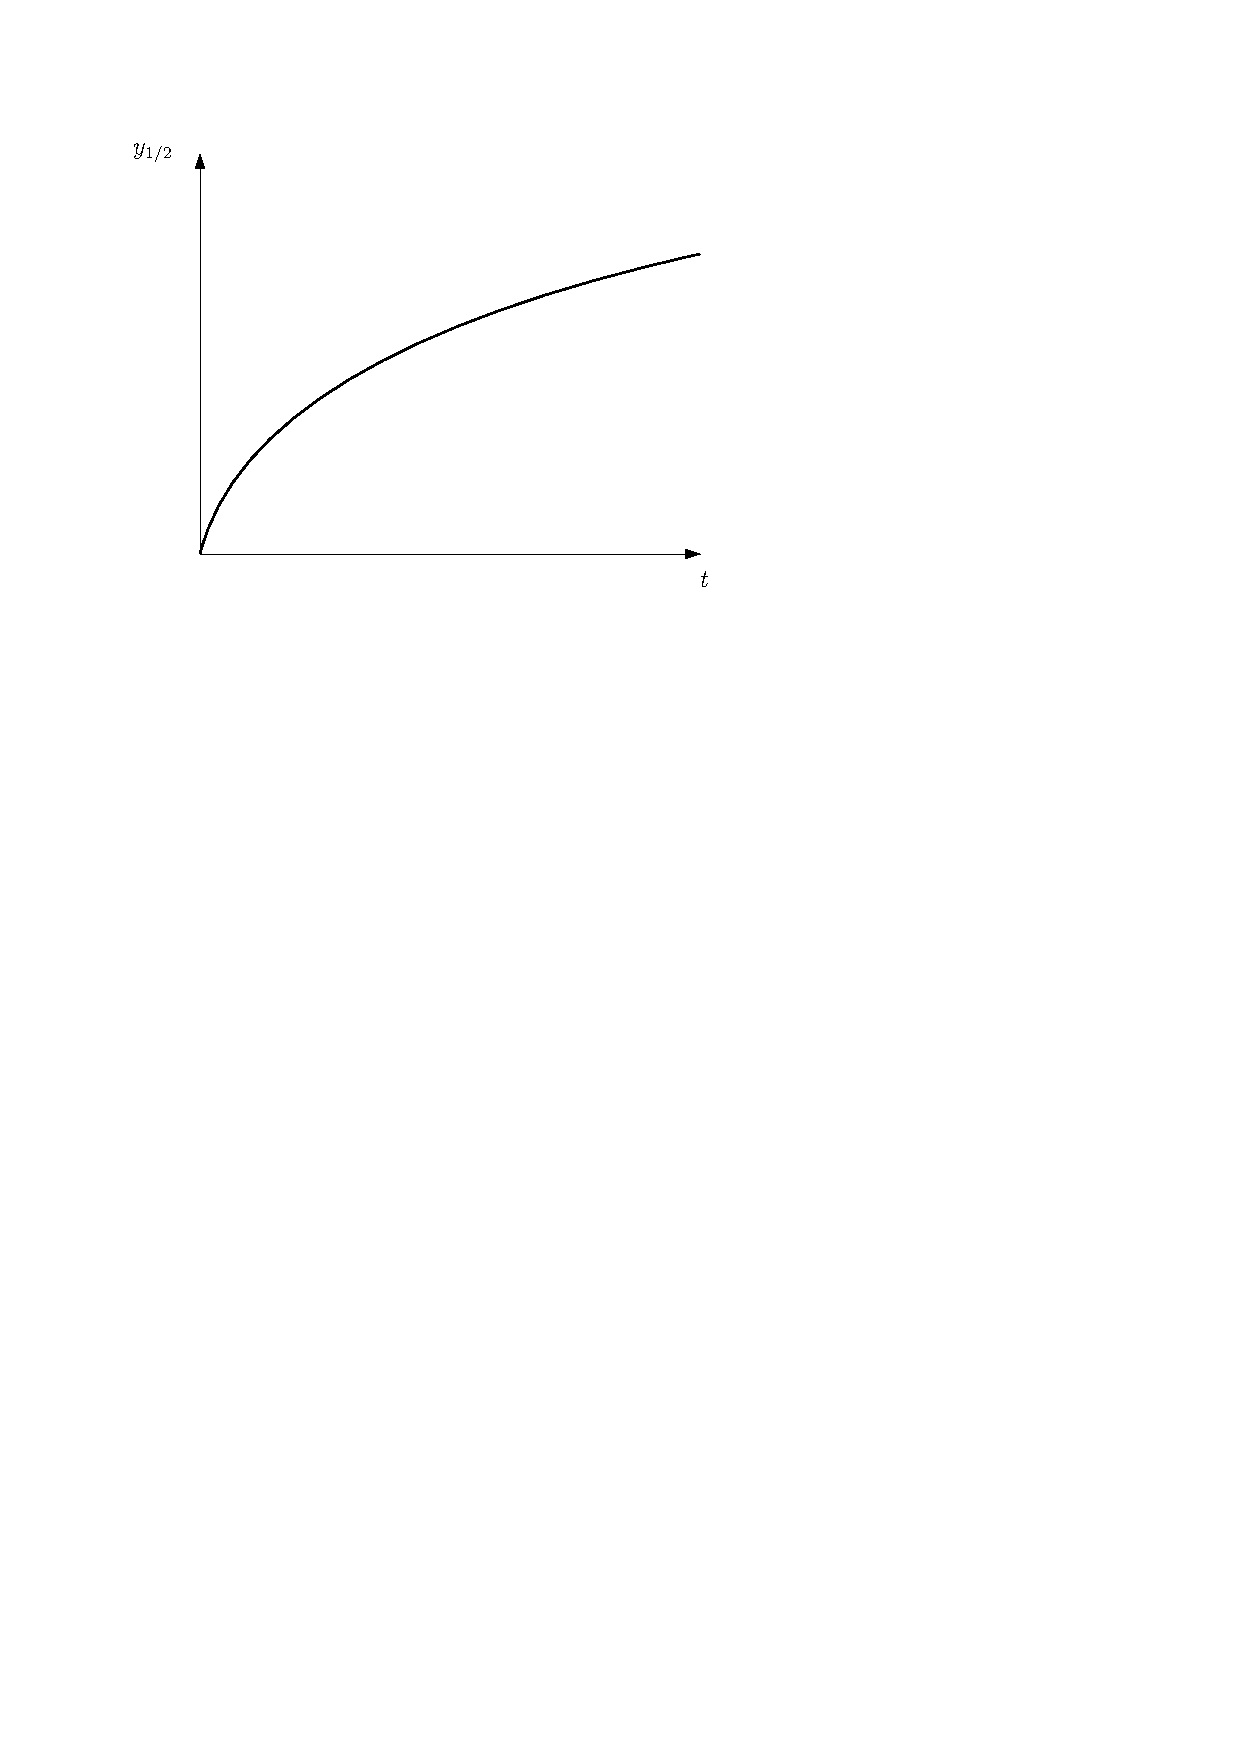
\includegraphics[scale=0.7]{./3.6 Soluzioni esatte equazioni di Navier-Stokes/3.6-13}
		\centering
		\caption{$y_{1/2}$ in funzione del tempo}
	\end{figure}
%
Per un oggetto reale questa approssimazione vale finché lo spessore è piccolo rispetto alla lunghezza della lastra.

È possibile calcolare lo sforzo sulla lastra come:
%
	\begin{equation*}
		\tau = \mu u_y = \frac{1}{h} f' = \frac{\mu U}{\sqrt{\nu t}} {\left[ 1 - \erf{\frac{z}{2}} \right]'}_{z=0} = - \frac{\mu U_1}{\sqrt{\nu t} 2 \sqrt{\pi}}
	\end{equation*}
%
Che può essere riscritto come:
%
	\begin{equation*}
		\tau = \rho {\nu}^{1/2} t^{-1/2} U \frac{1}{2 \sqrt{\pi}}
	\end{equation*}
%
Nonostante lo sforzo a zero tenda ad infinito, l'impulso\footnote{che è la variazione della quantità di moto}, che si calcola come integrale dello sforzo, rimane finito.
 %
	\begin{figure}[ht]
		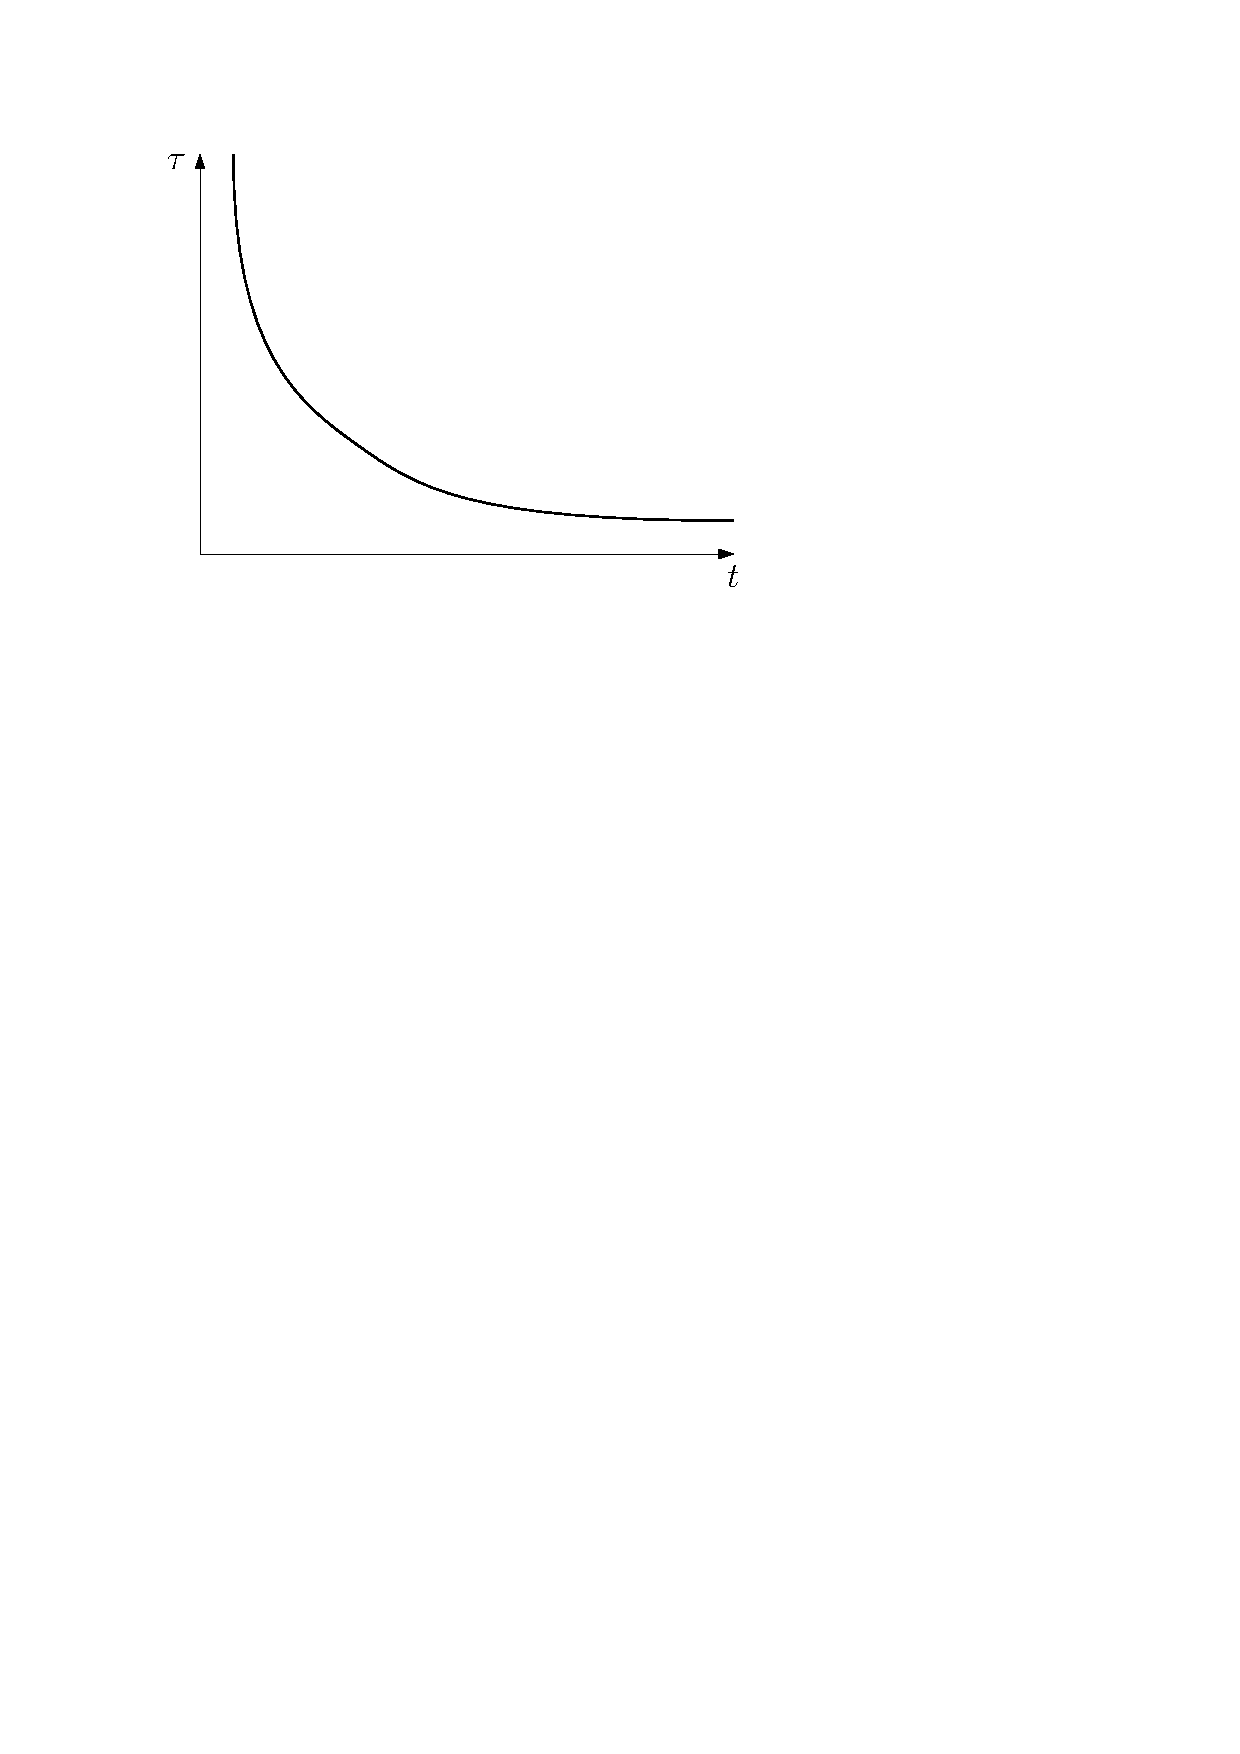
\includegraphics[scale=0.7]{./3.6 Soluzioni esatte equazioni di Navier-Stokes/3.6-14}
		\centering
		\caption{Grafico dello sforzo}
	\end{figure}
%
Si può calcolare la forza esercitata sulla lastra noti lo sforzo e l'area.

\subsection*{Bibliografia 3.7}
\cite[Cap.\ 9.5, 9.6]{CengelCimbala}\\
\cite[Cap.\ 6.1, 6.2, 6.3, 6.4, 6.5]{PnueliGutfinger}